\documentclass[UTF8,a4paper,10pt]{ctexart}
\usepackage[left=2.5cm, right=2.5cm, top=2.5cm, bottom=2.5cm]{geometry}


\usepackage{amsmath, amsfonts, amssymb} % math equations, symbols
\usepackage{lipsum}
\usepackage{color}      % color content
\usepackage{graphicx}   % import figures
\usepackage{url}        % hyperlinks
\usepackage{hyperref}   % bookmarks

\usepackage{xcolor}   % 导入xcolor包以使用颜色
% \usepackage{calc} % 用于计算长度
% \usepackage{markdown}

%使用listing包嵌入代码
\usepackage{listings} % 导入listings包
% \setlength{\tabwidth}{1cm}
\lstset{
  language=Mathematica, % 指定语言为Mathematica
  basicstyle=\ttfamily\small, % 设置基本样式
  keywordstyle=\bfseries, % 设置关键字样式
  commentstyle=\color{gray}, % 设置注释样式
  % stringstyle=\color{gray}, % 设置字符串样式
  showstringspaces=false, % 不显示字符串中的空格标记
  % frame=single, % 显示边框
  frame=L, % 显示边框
  xleftmargin=1cm,
  framexleftmargin=0cm,
  breaklines=true, % 自动换行
  % numbers=left, % 行号显示在左侧
  % numberstyle=\small, % 行号样式
  numbersep=10pt,% 行号与代码之间的间距
}


\renewcommand{\baselinestretch}{1.2}


\DeclareSymbolFont{greeks}{U}{eur}{m}{n}
\SetSymbolFont{greeks}{bold}{U}{eur}{b}{n}

\DeclareMathSymbol\eurmalpha  \mathord{greeks}{"0B}
\DeclareMathSymbol\eurmbeta  \mathord{greeks}{"0C}
\DeclareMathSymbol\eurmgamma  \mathord{greeks}{"0D}
\DeclareMathSymbol\eurmdelta  \mathord{greeks}{"0E}
\DeclareMathSymbol\eurmepsilon \mathord{greeks}{"0F}
\DeclareMathSymbol\eurmzeta  \mathord{greeks}{"10}
\DeclareMathSymbol\eurmeta  \mathord{greeks}{"11}
\DeclareMathSymbol\eurmtheta  \mathord{greeks}{"12}
\DeclareMathSymbol\eurmkappa \mathord{greeks}{"14}
\DeclareMathSymbol\eurmlambda  \mathord{greeks}{"15}
\DeclareMathSymbol\eurmmu  \mathord{greeks}{"16}
\DeclareMathSymbol\eurmnu  \mathord{greeks}{"17}
\DeclareMathSymbol\eurmxi  \mathord{greeks}{"18}
\DeclareMathSymbol\eurmpi \mathord{greeks}{"19}
\DeclareMathSymbol\eurmrho  \mathord{greeks}{"1A}
\DeclareMathSymbol\eurmsigma \mathord{greeks}{"1B}
\DeclareMathSymbol\eurmtau \mathord{greeks}{"1C}
\DeclareMathSymbol\eurmphi  \mathord{greeks}{"1E}
\DeclareMathSymbol\eurmchi \mathord{greeks}{"1F}
\DeclareMathSymbol\eurmpsi  \mathord{greeks}{"20}
\DeclareMathSymbol\eurmomega  \mathord{greeks}{"21}

\newcommand{\dsize}{\displaystyle}
\newcommand{\abs}[1]{\left\vert{#1}\right\vert}
\newcommand{\xx}{\hspace*{-.5pt}}
\newcommand{\yy}{\hskip7.5pt}
\newcommand{\zz}{\hskip9pt}
\newcommand{\be}{\begin{equation}}
\newcommand{\ee}{\end{equation}}
\newcommand{\rmd}{{\rm d}}
\newcommand{\gm}[1]{\Gamma \left( #1 \right)}
\newcommand{\res}{{\rm res}\, }
\newcommand{\vp}{{\rm v.p.}}
\newcommand{\dlim}{\dsize \lim}
\newcommand{\dsum}[2]{\dsize \sum_{#1}^{#2}}
\newcommand{\dint}{\dsize \int}
\newcommand{\doint}{\dsize \oint}
\newcommand{\dd}[2]{\dfrac {\rmd #1}{\rmd #2}}
\newcommand{\dif}[3]{\dfrac {{\rmd}^{#1} {#2}}{\rmd {#3}^{#1}}}
\newcommand{\pp}[2]{\dfrac {\partial #1}{\partial #2}}
\newcommand{\qq}[2]{\dfrac {{\partial}^2 #1}{\partial {#2}^2}}
\newcommand{\pq}[3]{\dfrac {{\partial}^2 #1}{\partial #2 \partial #3}}
\newcommand{\pqpq}[3]{\dfrac {{\partial}^{#1} #2}{\partial {#3}^{#1}}}
\newcommand{\call}[1]{{\cal L} \left \{ #1 \right \}}
\newcommand{\id}{{\it \Delta}}
\newcommand{\veps}{\varepsilon}
\newcommand{\rmi}{{\rm i}}
\newcommand{\rmpi}{\eurmpi}
\newcommand{\pii}{\rmpi \, \rmi}
\newcommand{\ipi}{\rmi \rmpi}
\newcommand{\example}[1]{{\bf 例12.{#1}}{\zz}}
\newcommand{\exmp}{{\bf 例}{\zz}}
\newcommand{\exer}[1]{{\bf 练习12.{#1}}{\yy}}
\newcommand{\answer}{{\bf 解}{\zz}}
\newcommand{\proof}{{\bf 证}{\zz}}
\newcommand{\lemma}[1]{{\bf 引理12.{#1}}{\zz}}
\newcommand{\lmm}{{\bf 引理}{\zz}}
\newcommand{\theorem}[1]{{\bf 定理12.{#1}}{\zz}}
\newcommand{\thrm}{{\bf 定理}{\zz}}
\newcommand{\property}[1]{{\bf 性质{#1}}{\zz}}
\newcommand{\col}[1]{{\bf 推论{#1}}{\zz}}
\newcommand{\cly}{{\bf 推论}{\zz}}
\newcommand{\ssum}[1]{\sum_{#1}^{\infty}}
\newcommand{\ddsum}[1]{\dsize \sum_{#1}^{\infty}}
\newcommand{\n}{n \to \infty}
\newcommand{\ddlim}{\dsize \lim_{\n}}
\newcommand{\dz}[1]{\dfrac {\rmd {#1}}{\rmd z}}
\newcommand{\ddz}[1]{\dfrac {{\rmd}^2 {#1}}{\rmd z^2}}
\newcommand{\dt}[1]{\dfrac {\rmd {#1}}{\rmd t}}
\newcommand{\ddt}[1]{\dfrac {{\rmd}^2 {#1}}{\rmd t^2}}
\newcommand{\lp}[1]{l_{#1}^{\prime}}
\newcommand{\pr}{\prime}
\newcommand{\ftnt}[2]{\!$^{\text{\zihao{6}{#1}}}$\afootnote"{}"{\zihao{6}{#1}{\hspace*{5pt}}{#2}}}
\newcommand{\pmpm}{\prime \prime}
\newcommand{\cdash}{\rule[3pt]{20pt}{.2mm}}
\newcommand{\Laplace}{{\nabla}^2}

\newcommand{\mma}{Mathematica}


\usepackage{listings}
\lstset{language=Mathematica}

\title{Wolfram Mathematica 在数学物理方法课程中的应用}
\author{}
\date{}

\begin{document}
\maketitle


Wolfram Mathematica~是一款符号计算软件,
% 有时候也被称为计算机代数系统,
广泛使用于科学、工程、数学、计算等领域。经
过30多年的发展,截止2024年已经到了版本14,功能已经得到了极大的扩充,
除了强大的符号与数值计算功能如微积分、幂级数展开、线性代数计算、
求解微分方程、积分变换等之外,也可以进行并行计算、GPU计算,还能搭
建神经网络、进行机器学习。使用Wolfram Alpha知识搜索引擎,Mathematica还能进行地理、
金融、社会、语言等各方面的计算,号称为“全球现代技术计算的终极系统”。限于篇幅
,本章只介绍与本课程内容相关的内容。

在目前的数学软件中,Mathematica的帮助文档是最好的之一。其帮助文档内置了《虚拟全书》
,这是一份官方的入门
教程。《虚拟全书》可以通过在帮助文档地址栏输入
\href{http://reference.wolfram.com/language/tutorial/VirtualBookOverview.html}{tutorial/VirtualBookOverview}
进入,或者直接在地址栏搜索“虚拟全书”。而且Mathematica帮助文档可以直接在上面进行代码的修改和运行,中文版软件的帮助文档绝大部分内容
已经翻译,降低了学习的难度。此外中文版的帮助文档还支持输入中文内容进行搜索。在学
习Mathematica的过程中,应该经常查阅帮助文档。学习以下内容时,请打开软件运行例子并时刻查询帮助文
档。以下所遇见的函数不做具体用法说明,请读者自行用鼠标选定函数按~\fbox{F1}~键查询其用法。

另外,用于Mathematica的编程语言是一种严谨且优雅的语言,称为Wolfram 语言。
Wolfram语言同时含有面向过程编程和函数式编程,但函数式编程在Mathematica里面更加方便,
运行速度也更快,也更符合Wolfram语言的编程风格。
想要深入了解的读者,可以参考帮助文档\href{http://reference.wolfram.com/language/tutorial/CoreLanguageOverview.html}{tutorial/CoreLanguageOverview}。
以下内容可能涉及一点Mathematica语法的内容,出现时只做简单介绍。在下面的举例中,输入和输出的
内容都尽量与屏幕显示的格式一致,但也存在一些不同之处。本文附有一个 Mathematica notebook 文件,包含本文中所有的可运行代码。本文中很多绘图的结果不在本文中展示,请读者自行参考代码文件。


\begin{figure}[htbp]
\centering
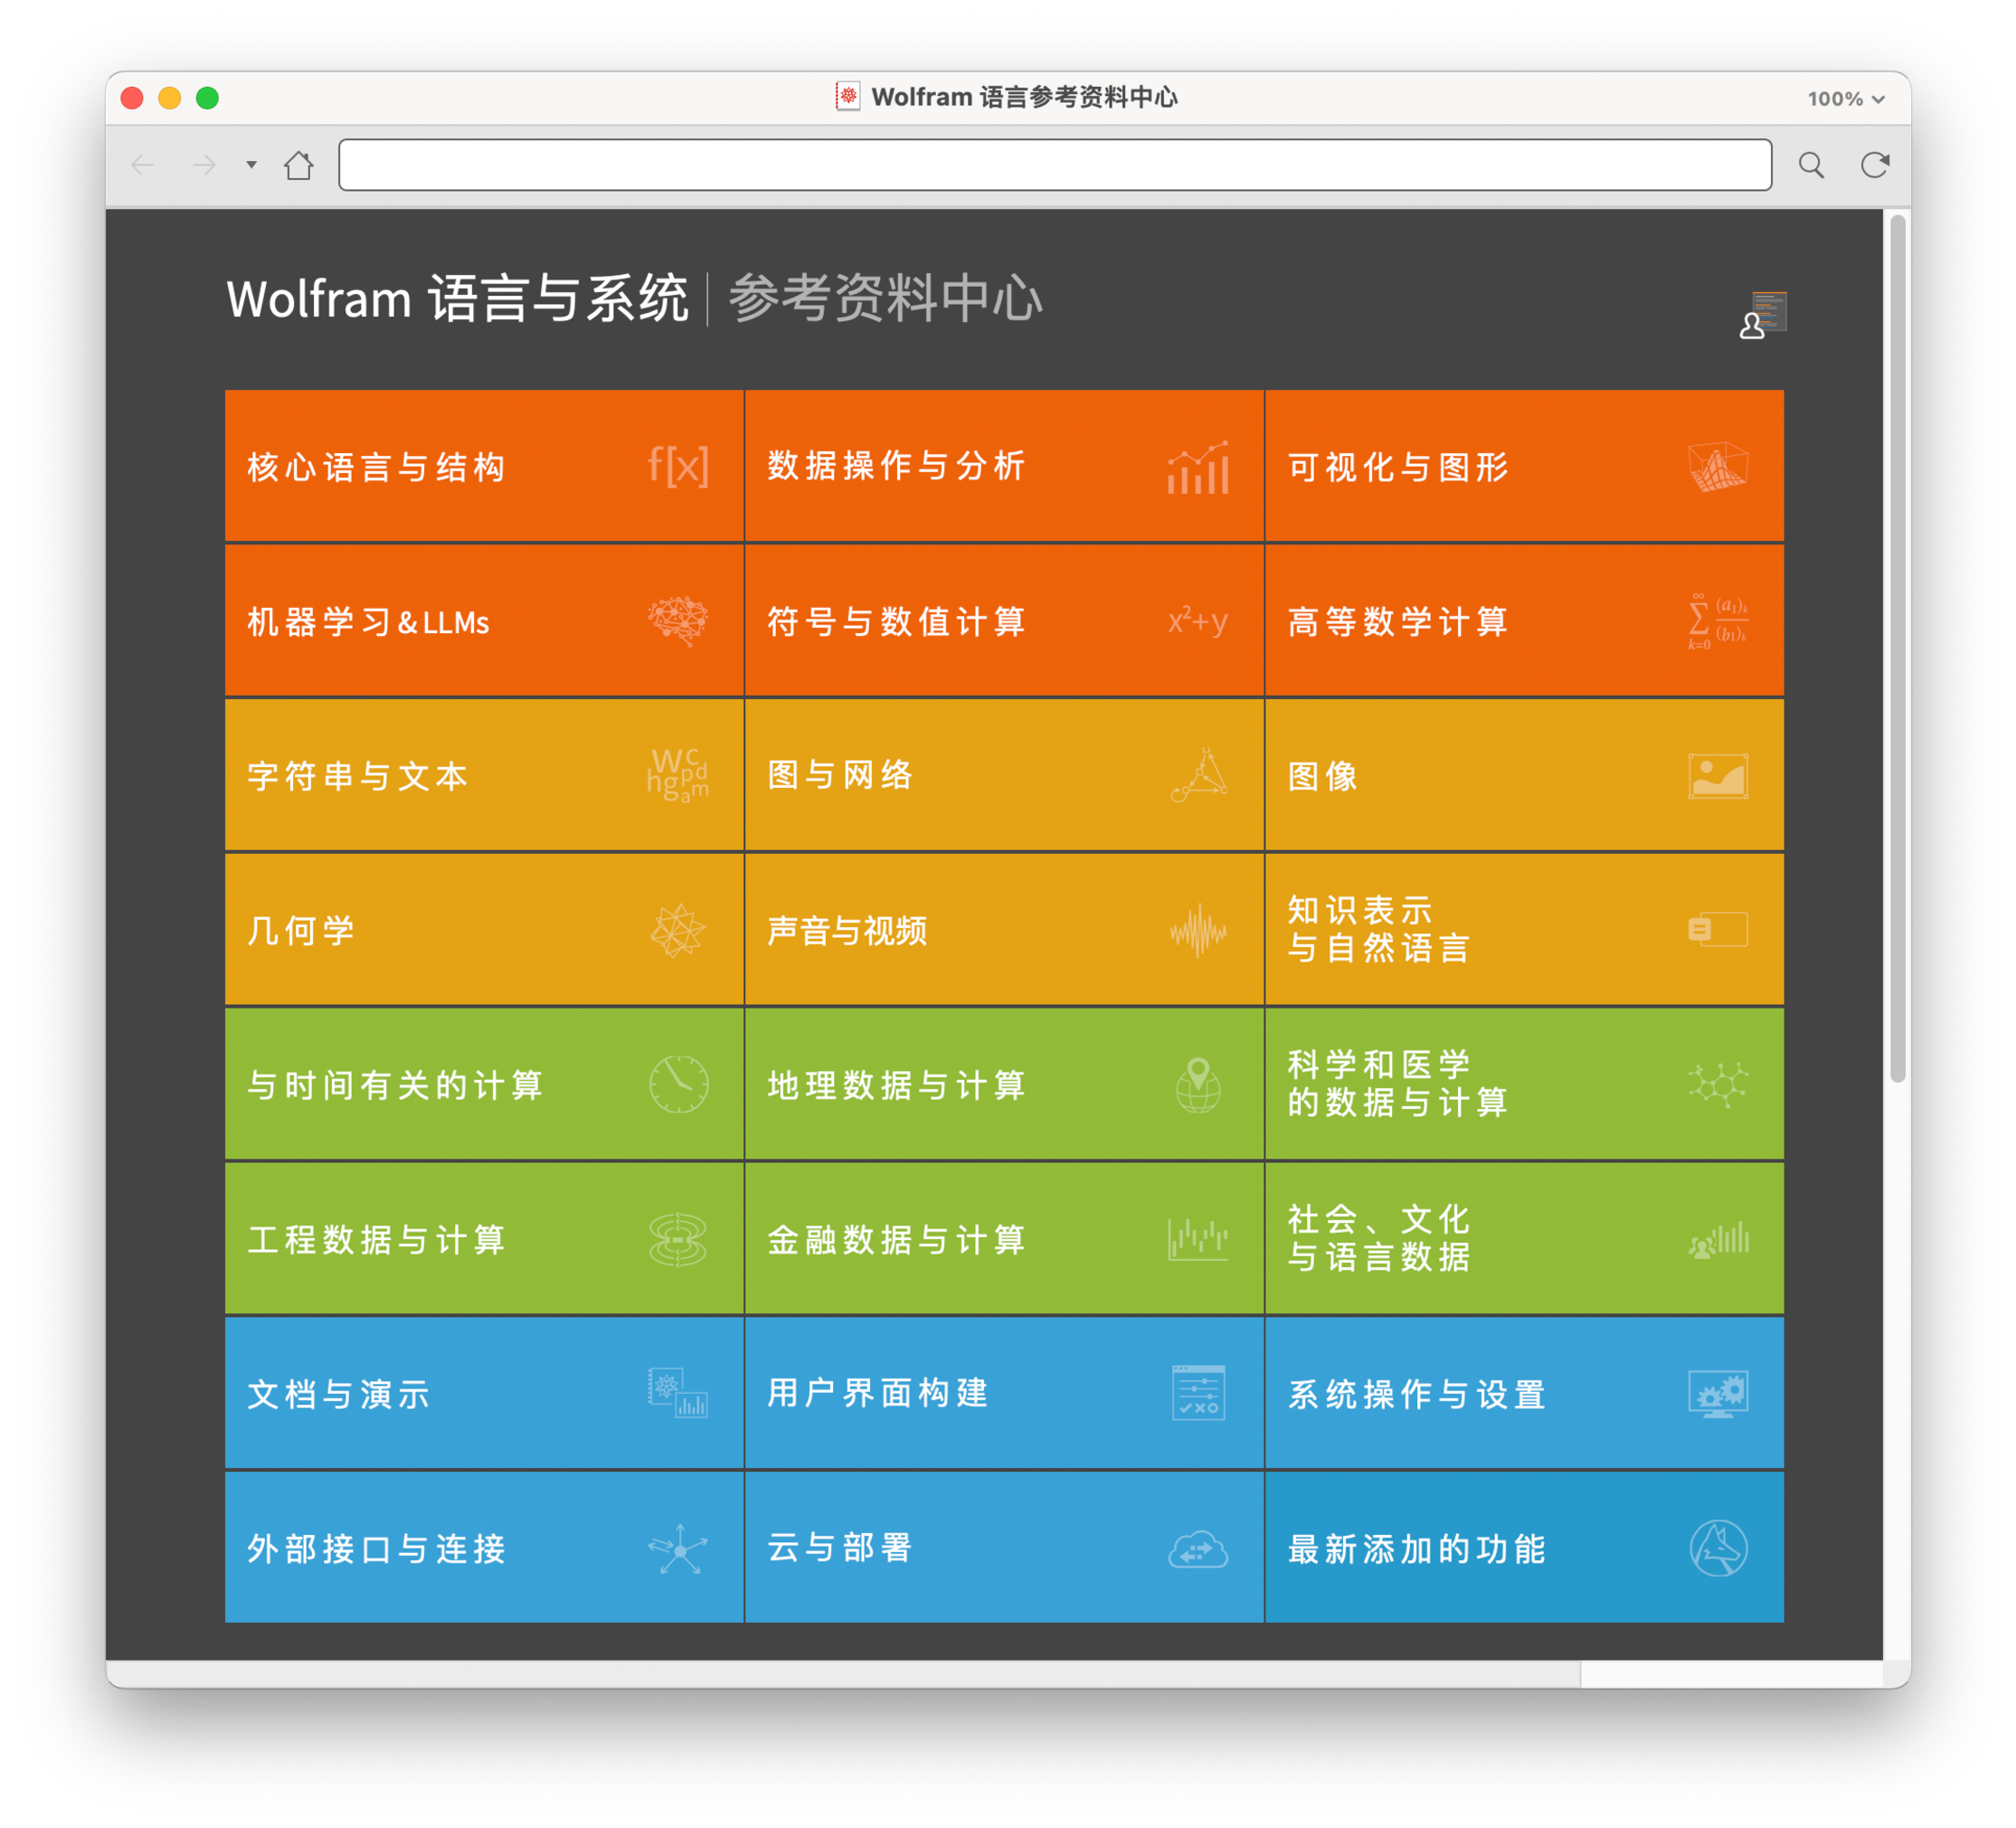
\includegraphics[height=9cm]{img/DocMain.pdf}
\caption{Mathematica帮助文档首页}
% \label{figure}
\end{figure}


% {\centering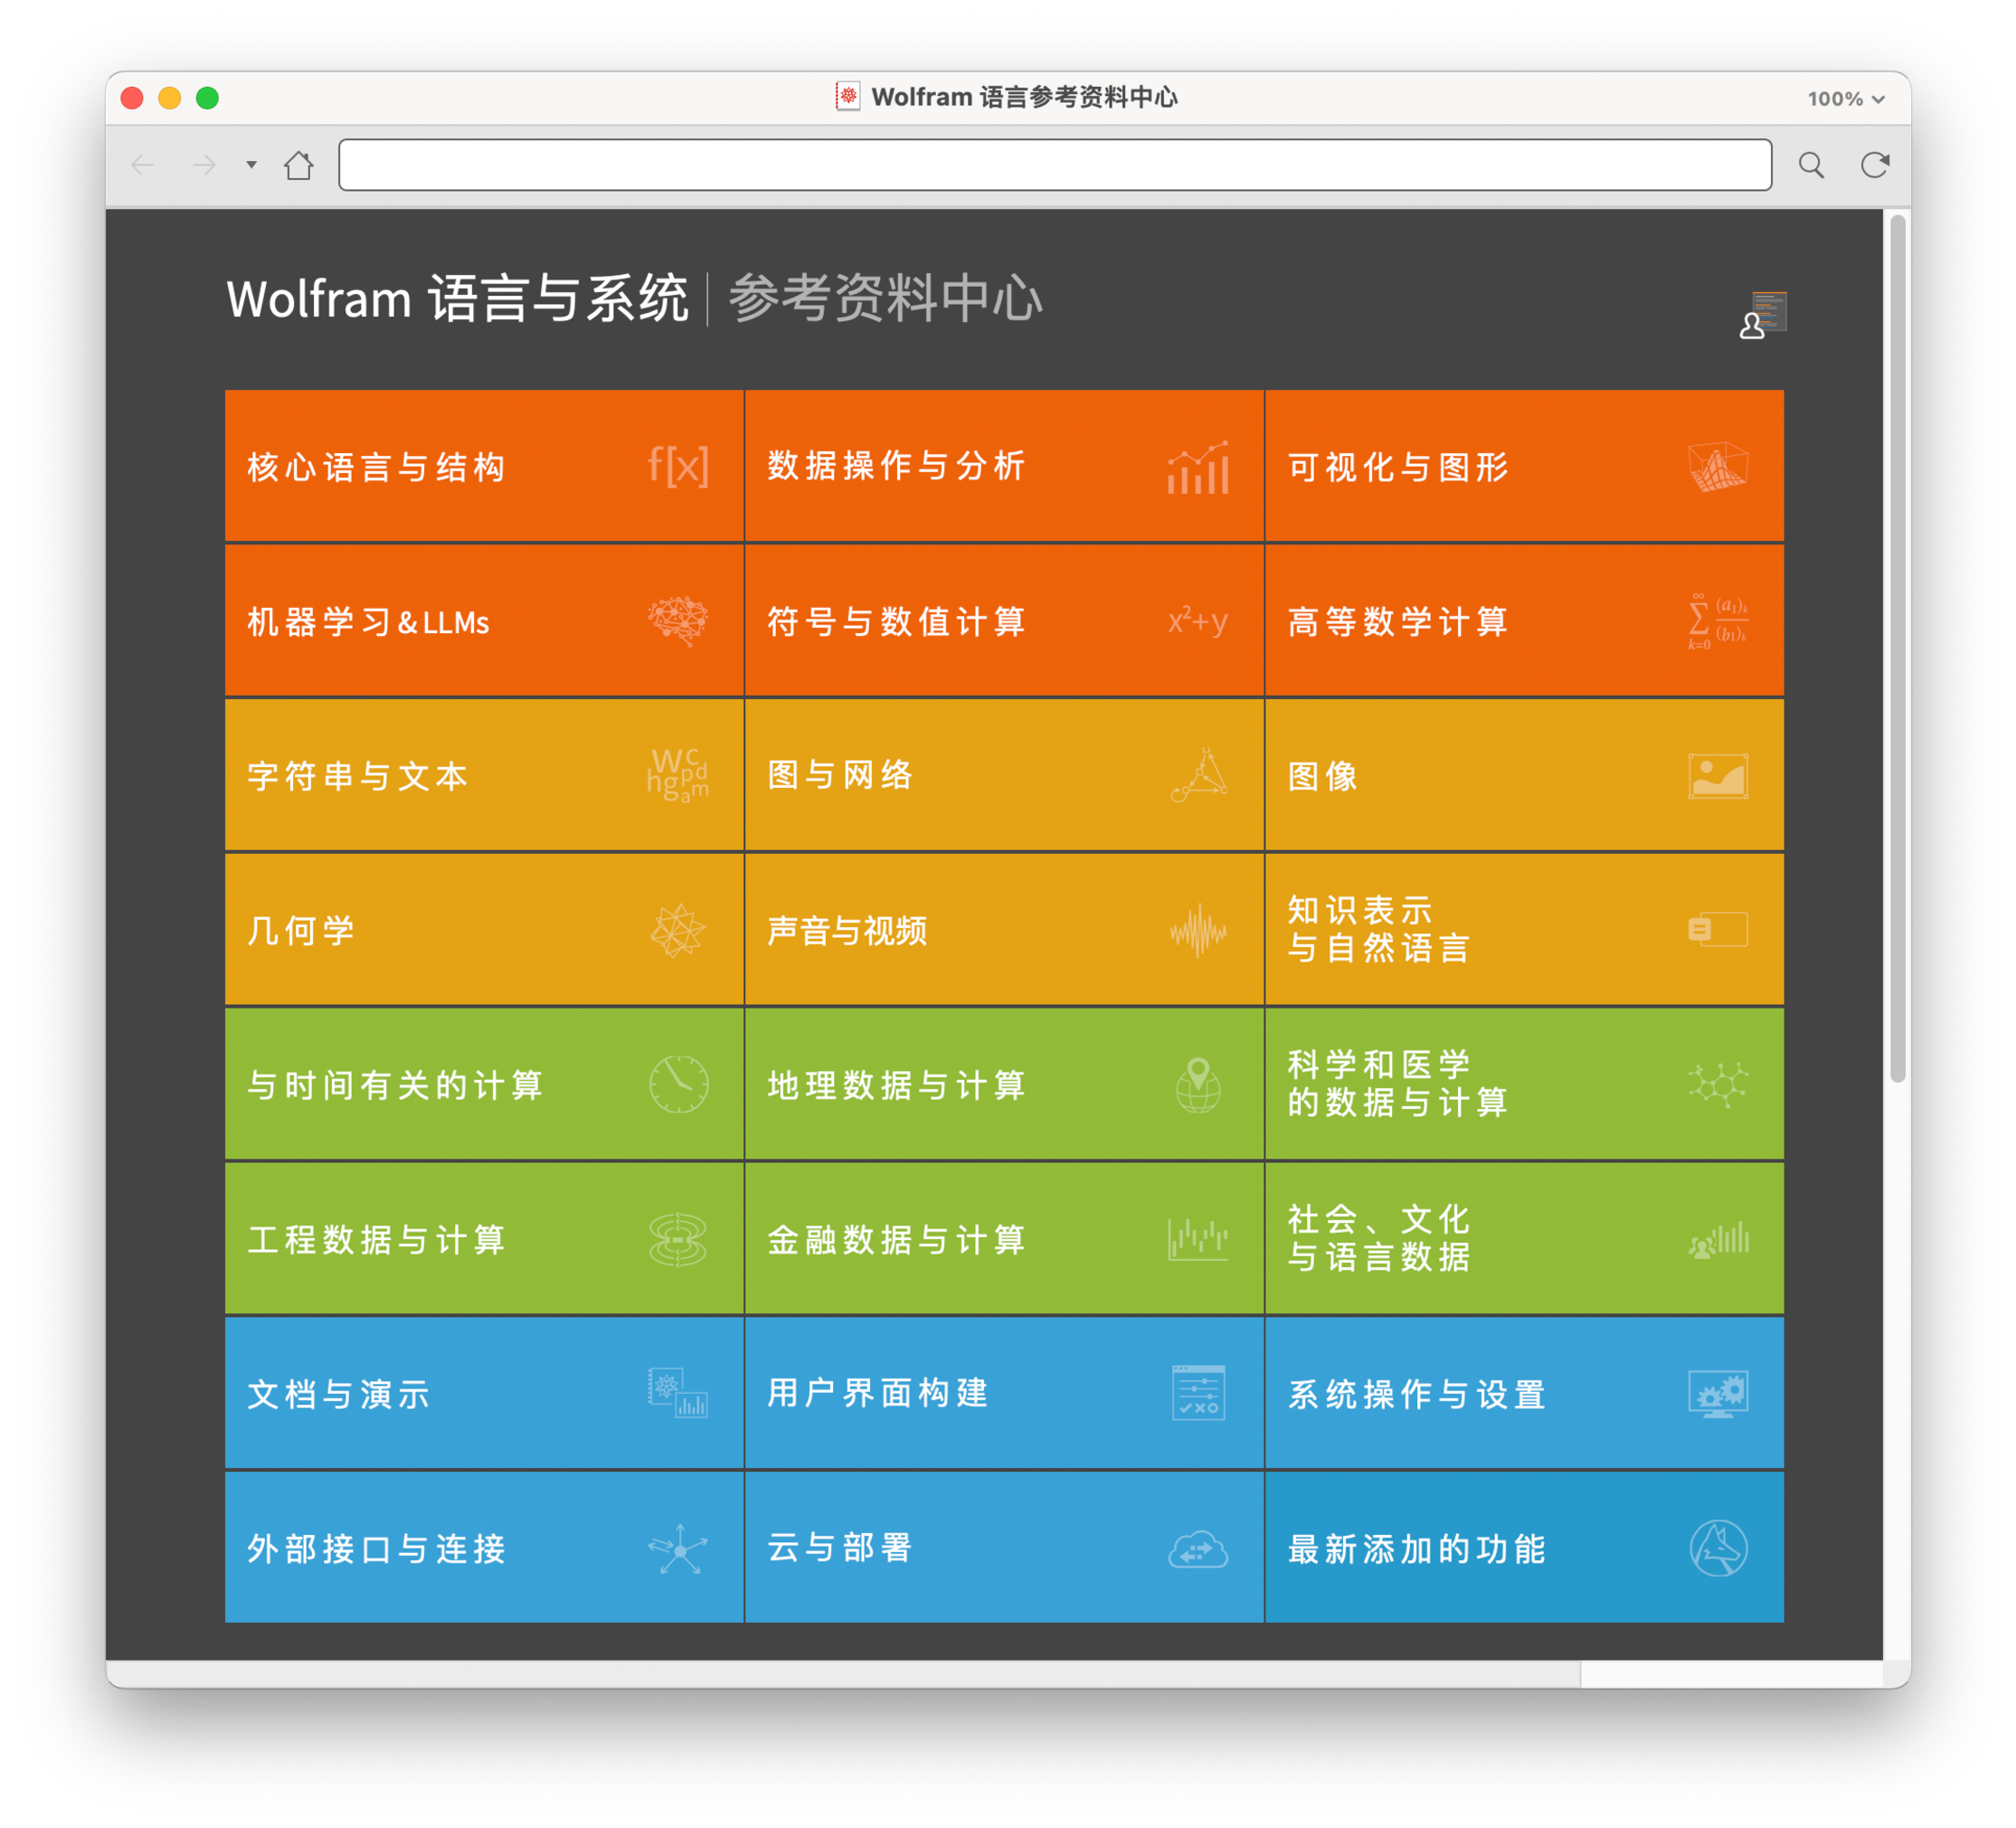
\includegraphics[height=8cm]{img/DocMain.pdf}}
% \centerline{{图1.Mathematica帮助文档首页}}
% \vspace*{7.5pt}
% %\begin{minipage}[b]{6.5cm}\parindent=2\ccwd
% %\end{minipage}
% %\newpage

\section{Mathematica 基础知识}
以下内容只是简单的介绍,详见帮助文档
\href{http://reference.wolfram.com/language/tutorial/IntroductionOverview.html}{tutorial/IntroductionOverview}。

% \begin{lstlisting}
% (* Mathematica code *)
% f[x_] := Sin[x] + Cos[x]
% Plot[f[x], {x, 0, 2 Pi}]
% \end{lstlisting}

\subsection{进行输入和计算}

Mathematica可以直接当作计算器使用。打开Mathematica,新建一个笔记本(.nb)文件,就可以进行表达式的输入和计算。把光标移动到笔记本窗口内,键入要操作的表达式,如

\verb|1+1|

然后按下\fbox{Shift+Enter}或者小键盘的\fbox{Enter} ,就会在显示屏上显示:

\verb|In[1]:=1+1|

\verb|Out[1]=2|

其中In[1]和Out[1] 是自动出现的,表示第1次的计算结果。若想重用以前的计算结果,
可以使用~\verb|%|~调用,其中~\verb|%|~表示前一个计算的结果,\verb|%%|~表示倒数第二个计算的结果,\verb|%n|~表示第n个计算的结果:

\verb|In[2]:=Sqrt[%]|

\verb|Out[2]=|$\sqrt{2}$

\verb|In[3]:=N[%2]|

\verb|Out[3]=1.41421|

除了一般的输入,Mathematica还支持二维输入,比如按下\fbox{Ctrl + 2}键直接输入根号,\fbox{Ctrl + /}键输入二维的分号,
或者在\emph{面板——数学助手}里面点击输入二维表达式。想要了解更多的二维表达式输入,可以参考帮助文档\href{http://reference.wolfram.com/language/tutorial/TwoDimensionalExpressionInput.html}{tutorial/TwoDimensionalExpressionInput}。

\subsection{算术运算符号}
+(加号,\verb|Plus|),-(减号,\verb|Subtract|),*(乘号,\verb|Times|),/(除号,\verb|Divide|), $\hat{}$(乘方,\verb|Power|)。此外*可以用空格代替,**(\verb|NonCommutativeMultiply|)表示没有交换律的乘号,通常用于四元数的运算以及自定义算符的运算中。

\subsection{数与数学常数}
Mathematica中数包括整数、有理数、实数、复数。在计算表达式的过程中,除非遇到小数,否则Mathematica 会给出精确结果:

\verb|In[1]:=Sqrt[3]|

\verb|Out[1]=|$\sqrt{3}$

\verb|In[2]:=Sqrt[3.]|

\verb|Out[2]:=1.73205|

如果想要得到近似值的话,Mathematica的函数~\verb|N|~可以给出任意精度的近似解,如:

\verb|In[3]:=N[Pi,100]|

\verb|Out[3]=3.141592653589793238462643383279502884197169399375105820974944592307816|\\
\verb|       406286208998628034825342117068|

\mma 也可以指定输入的数的精度,比如~\verb|3.1`30|~就代表精确度为30的数,再如

\verb|In[4]:=3.1`30 + 2.1`20 + 1|   

\verb|Out[4]:=6.2000000000000000000|   

由于参与计算的三个数精确度依次是30、20和无穷大,所以最后给了精确度为20左右的结果。更多信息参考函数~\verb|Precision|~和~\verb|Accuracy|。      

Mathematica中虚数的单位是大写的I,$\pi$为Pi,自然对数底数$e$为E,如

\verb|In[5]:=E^(1+Pi I)|

\verb|Out[5]=|$-e$

Mathematica中还有其他常数,具体见帮助文档
\href{http://reference.wolfram.com/language/tutorial/MathematicalConstants.html}{tutorial/MathematicalConstants}
,下面列举了一些常用的常数:
\noindent
\tabcolsep=2pt
\begin{center}
\begin{tabular}{ll|cl|ll}
\hline\hline\hline
\makebox[1.35cm][c]{} & \makebox[2.65cm][l]{} &
\makebox[.5cm][c]{} & \makebox[2.75cm][l]{} &
\makebox[3.5cm][c]{} & \makebox[2cm][l]{} \\[-12pt]
\;\verb+Pi+ & {\;}圆周率$\pi$ &
\verb+E+ & {\;}自然对数的底e &
\;\verb+EulerGaMathematica+ & {\;}欧拉常数$\gamma$ \\
\;\verb+Degree+ & {\;}角度单位$\rmpi / 180$ &
\verb+I+ & {\;}虚单位i &
\;\verb+Infinity, -Infinity+ & {\;\;\,}$\infty, -\infty$ \\
\hline\hline\hline
\end{tabular}
\end{center}

除了用上述列表中的方式输入数学常数外,\mma 还有额外的输入方式。比如圆周率\verb|Pi|的输入方式为依次按下键盘的~\fbox{ESC}~\fbox{P}~\fbox{I}~\fbox{ESC},虚数\verb|I|的输入方式为~\fbox{ESC}~\fbox{I}~\fbox{I}~\fbox{ESC},无穷大\verb|Infinity|为
~\fbox{ESC}~\fbox{I}~\fbox{N}~\fbox{F}~\fbox{ESC}。更多相关可以参考帮助文档
\href{http://reference.wolfram.com/language/tutorial/MathematicalAndOtherNotation.html}{tutorial/MathematicalAndOtherNotation}。



\subsection{Mathematica中的括号}

Mathematica中有四种括号:表示运算级别的小括号\verb|( )|,表示函数的方括号\verb|[ ]|(\verb|f[x]|),表示列表的花括号  \verb|{ }|(\verb|{a, b, c}| ),以及表示列表索引的双括号\verb|[[ ]]|(\verb|{a, b, c} [[1]]|)。

\subsection{Mathematica中的函数}

作为一种函数式编程语言,Mathematica中所有对象都是表达式(见
\href{http://reference.wolfram.com/language/tutorial/ExpressionsOverview.html}{tutorial/ExpressionsOverview}
),函数是Mathematica的基础。Mathematica中函数名或者变量名为字符串,中
间不能有空格(否则认为是两个符号相乘),不能有下划线(否则认为是模式,模式见
\href{http://reference.wolfram.com/language/tutorial/PatternsOverview.html}{tutorial/PatternsOverview}),不能以数字开头(否则认为是乘积,如2a会当做2和a的乘积),不能有小数点(否则认为是矩阵点积~\verb|Dot|)。
一般Mathematica中内置函数以首字母是大写的驼峰命名法命名,而且通常是英文单词的全拼。

Mathematica中的函数的调用一般是\verb|Func[x1,x2,...,|options\verb|->|values\verb|,...]|的形式,其中Func为函数名,
\verb|x1,x2|等为参数,参数可以为任意对象(比如数字,函数,代数表达式,图片等),
options\verb|->|values 是选项,通常用于限定函数的行为模式,比如限定算法或者绘图样式等。

初等数学函数,参见帮助文档
\href{http://reference.wolfram.com/language/guide/ElementaryFunctions.html}{guide/ElementaryFunctions}
,这里列举一些如下:
\par
\tabcolsep=2pt
\begin{center}
\begin{tabular}{lllllll|l}
\hline\hline\hline
& & & & & & & \\[-12pt]
\verb+Sqrt[z]+    & \verb+z^s+        &                   &
                  &                   &                   & \qquad & {\;}幂函数 \\
\verb+Exp[z]+     & \verb+Log[z]+     & \verb+Log[b, x]+  &
\verb+Log10[x]+   & \verb+Log2[x]+    &                   & \qquad & {\;}指数函数, 对数函数   \\
\verb+Sin[z]+     & \verb+Cos[z]+     & \verb+Tan[z]+     &
\verb+Cot[z]+     & \verb+Sec[z]+     & \verb+Csc[z]+     & \qquad & {\;}三角函数   \\
\verb+ArcSin[z]+  & \verb+ArcCos[z]+  & \verb+ArcTan[z]+  &
\verb+ArcCot[z]+  & \verb+ArcSec[z]+  & \verb+ArcCsc[z]+  & \qquad & {\;}反三角函数 \\
\verb+Sinh[z]+    & \verb+Cosh[z]+    & \verb+Tanh[z]+    &
\verb+Coth[z]+    & \verb+Sech[z]+    & \verb+Csch[z]+    & \qquad & {\;}双曲函数           \\
\verb+ArcSinh[z]+ & \verb+ArcCosh[z]+ & \verb+ArcTanh[z]+ &
\verb+ArcCoth[z]+ & \verb+ArcSech[z]+ & \verb+ArcCsch[z]+ & \qquad & {\;}反双曲函数 \\
\hline\hline\hline
\end{tabular}
\end{center}
%\pagebreak


特殊函数见帮助文档
\href{http://reference.wolfram.com/language/guide/SpecialFunctions.html}{guide/SpecialFunctions}
,广义函数见
\href{http://reference.wolfram.com/language/guide/GeneralizedFunctions.html}{guide/GeneralizedFunctions}
,这里列举一些如下:

\par
\tabcolsep=2pt
\noindent
\begin{center}
\begin{tabular}{p{9cm}l|lp{5cm}}
\hline\hline\hline
& & & \\[-13pt]
\verb+UnitStep[x]+                    & \qquad & & $\eta$函数(亥维赛的单位阶跃函数)\\[-0.20pt]
\verb-Gamma[z]-                       & \qquad & & $\Gamma$函数$\Gamma (z)$ \\[-0.20pt]
\verb-Beta[p, q]-                     & \qquad & & B函数${\rm B} (p, q)$ \\[-0.20pt]
\verb-PolyGamma[z]-                   & \qquad & & $\eurmpsi$函数$\eurmpsi (z)$ \\[-0.20pt]
\verb+MoebiusMu[n]+                   & \qquad & & 默比乌斯函数$\eurmmu (n)$ \\[-0.20pt]
\verb-Zeta[z]-                        & \qquad & & 黎曼$\eurmzeta$函数$\eurmzeta (z)$ \\[-0.20pt]
\verb-Erf[z]-                         & \qquad & & 误差函数${\rm erf} (z)$ \\[-0.20pt]
\verb-Erfc[z]-                        & \qquad & & 余误差函数${\rm erfc} (z)$ \\[-0.20pt]
\verb-LegendreP[n, x]-                & \qquad & & 勒让德多项式${\rm P}_n (x)$ \\[-0.20pt]
\verb-LegendreP[nu, x], LegendreQ[nu, x]-
                                      & \qquad & & 勒让德函数${\rm P}_{\nu} (x), \; {\rm Q}_{\nu} (x)$ \\[-0.20pt]
\verb-LegendreP[nu, mu, x], LegendreQ[nu, mu, x]-
                                      & \qquad & & 连带勒让德函数${\rm P}_{\nu}^{\mu} (x), \; {\rm Q}_{\nu}^{\mu} (x)$ \\[-0.20pt]
\verb-SphericalHarmonicY[l, m, u, v]- & \qquad & & 球面调和函数${\rm Y}_l^m (u, v)$ \\[-0.20pt]
\verb-BesselJ[nu, z], BesselY[nu, z]- & \qquad & & 贝塞耳函数${\rm J}_{\nu} (z), \; {\rm N}_{\nu} (z)$ \\[-0.20pt]
\verb-BesselI[nu, z], BesselK[nu, z]- & \qquad & & 虚宗量贝塞耳函数${\rm I}_{\nu} (z), \; {\rm K}_{\nu} (z)$ \\[-0.20pt]
\verb-AiryAi[z],- \; \verb-AiryBi[z]- & \qquad & & 艾里函数${\rm Ai} (z), \; {\rm Bi} (z)$ \\[-0.20pt]
\verb-SinIntegral[z]-                 & \qquad & & 正弦积分${\rm Si} (z)$ \\[-0.20pt]
\verb-CosIntegral[z]-                 & \qquad & & 余弦积分${\rm Ci} (z)$ \\[-0.20pt]
\verb-SinhIntegral[z]-                & \qquad & & 双曲正弦积分${\rm Shi} (z)$ \\[-0.20pt]
\verb-CoshIntegral[z]-                & \qquad & & 双曲余弦积分${\rm Chi} (z)$ \\[-0.20pt]
\verb-ExpIntegralEi[z], ExpIntegralE[n, z]-    & \qquad & & 指数积分${\rm Ei} (z), \; {\rm E}_n (z)$ \\[-0.20pt]
\verb-LogIntegral[z]-                 & \qquad & & 对数积分${\rm li} (z)$ \\[-0.20pt]
\verb-FresnelC[z], FresnelS[z]-       & \qquad & & 费涅耳积分${\rm C} (z), \, {\rm S} (z)$\\[-0.20pt]
\verb-GegenbauerC[n, m, z]-           & \qquad & & 盖根鲍尔多项式${\rm C}_n^{(m)} (z)$   \\[-0.20pt]
\verb-ChebyshevT[n, z], ChebyshevU[n, z]-     & \qquad & & 切比雪夫多项式${\rm T}_n (z), \; {\rm U}_n (z)$ \\[-0.20pt]
\verb-JacobiP[n, a, b, z]-           & \qquad & & 雅可比多项式${\rm P}_n^{(a, b)} (z)$    \\[-0.20pt]
\verb-HermiteH[n, z]-                & \qquad & & 厄米多项式${\rm H}_n (z)$            \\[-0.20pt]
\verb-LaguerreL[n, z], LaguerreL[n, a, z]-    & \qquad & & 拉盖尔多项式${\rm L}_n (z), \; {\rm L}_n^{\alpha} (z)$           \\[-0.20pt]
\verb-Hypergeometric2F1[a, b, c, z]- & \qquad & & 超几何函数${\rm F}(a, b; c; z)$         \\[-0.20pt]
\verb-Hypergeometric1F1[a, b, z]-    & \qquad & & 合流超几何函数${\rm F}(a; b; z)$        \\[2pt]
\hline\hline\hline
\end{tabular}
\end{center}

关于Mathematica内置的符号计算和画图的函数,将在后文一一介绍。

自定义函数(详见
\href{http://reference.wolfram.com/language/tutorial/TransformationRulesAndDefinitionsOverview.html}{tutorial/TransformationRulesAndDefinitionsOverview}
):Mathematica中最常见的自定义函数的方式如下:

\noindent
\begin{center}
\begin{tabular}{p{7cm}l|lp{5cm}}
\hline\hline\hline
& & & \\[-13pt]
\verb+f[x_]:=exp+                    & \qquad & & 定义一元函数 \\[-0.20pt]
\verb-f[x_,y_,z_,...]:=exp-        & \qquad & & 定义多元函数 \\[-0.20pt]
\hline\hline\hline
\end{tabular}
\end{center}
如:

\verb|In[1]:=f[x_]:=x^2|

\verb|In[2]:=f[a]|

\verb|Out[2]=|$\text{a}^2$

\verb|In[3]:=g[x_,y_]:=x y|

\verb|In[4]:=g[2,x]|

\verb|Out[4]=2 x|


\subsection{Mathematica中变量的清除}

很多时候,因为有些变量已经经过了赋值,如果没有注意的话可能会报错或者得不到想要的结果,比如运行以下代码就会报错:

% \verb|In[1]:=x=1;Integrate[x Sin[x], x]|

\begin{lstlisting}
x=1;
Integrate[x Sin[x], x]
\end{lstlisting}

这时候就要清除变量x:
\begin{lstlisting}
Clear[x];
Integrate[x Sin[x], x]
(*-x Cos[x] + Sin[x]*)
\end{lstlisting}

% \verb|In[2]:=Clear[x];Integrate[x Sin[x], x]|

% \verb|Out[2]=-x Cos[x] + Sin[x]|

另外,想要清除所有变量,可以运行\verb|Clear["Global`*"]|,或者在菜单~\emph{ 计算—退出内核—Local}~
退出内核再~\emph{ 计算—启动内核—Local}~启动内核,这样之前所有的定义就会清空。


\subsection{Mathematica初学者应该注意的事情}

初学者比较容易犯的错误是将\mma 当作一个高级计算器而忽视了\mma 其实也是一门严谨的编程环境,以下总结了初学者应注意的事情:(1)不能乱用括号;(2)不能混淆中文逗号和英文逗号,使用中文逗号的常见结果是Mathematica把中文逗号当做
一个符号与逗号前后的内容相乘;(3)内置函数首字母一定要大写;
(4)注意=和==的区别,=是赋值(Set),==是相等(Equal);(5)在对Mathematica的语法不是非常了解的情况下,不要使用下标 (Subscript);
(6)注意Mathematica界面代码的颜色,其中黑色是已赋值的函数或者变量,特别的,内置函数一定是黑色的;绿色是局部变量,
红色是错误提示。注意这些点能够避免很多错误。

\section{Mathematica 的语言结构}

\mma 是一门函数式编程语言,里面的一切对象都是表达式。
比如\verb|a=1|这个赋值语句在Mathematica中其实是表达式\verb|Set[a,1]|,
定义函数的语句\verb|f[x_]:=x^2|的完整形式是

% \verb|SetDelayed[f[Pattern[x, Blank[]]], Power[x, 2]]|
\begin{lstlisting}
SetDelayed[f[Pattern[x, Blank[]]], Power[x, 2]]
\end{lstlisting}

\noindent
在\mma 中,我们可以用函数\verb|FullForm|来查看一个表达式的完整形式,如

\verb|In[1]:=FullForm[Hold[f[x_] := x^2]]|

\verb|Out[1]=Hold[SetDelayed[f[Pattern[x, Blank[]]], Power[x, 2]]]|

\noindent
这里\verb|Hold|的作用是让里面的表达式不进行运算。此外我们可以通过函数\verb|TreeForm|来查看一个表达式的结构树,如

\verb|In[2]:=TreeForm[Hold[f[x_] := x^2]]|

\begin{minipage}[b]{0.0cm}
\verb|Out[2]=|
\\\\\\\\%为了调纵向居中,我才不会告诉你我试了半天最终以四个回车解决了:)
\end{minipage}
\hfill
\begin{minipage}[b]{14.3cm}\parindent=2\ccwd
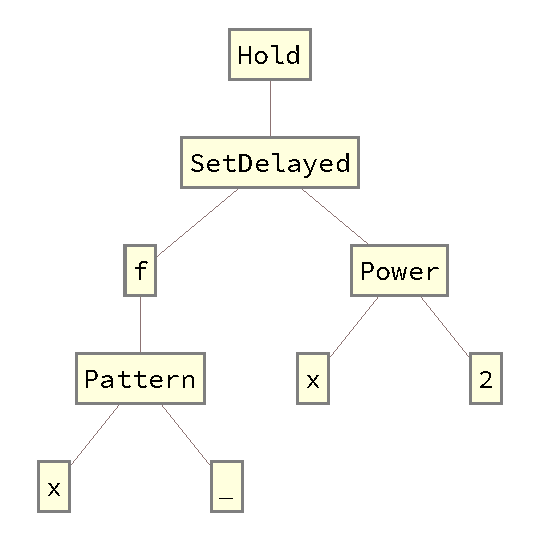
\includegraphics[height=4cm]{img/TreeForm.pdf}
\end{minipage}

\noindent
\mma 中一切皆表达式的含义远远不止如此,很多编程语言中的所谓语法在\mma 中都是表达式的一种语法糖。比如\mma 中依次运算几个语句需要用“\verb|;|”隔开,实际上这种使用方式是函数~\verb|CompoundExpression|~的语法糖,我们可以用鼠标选中“\verb|;|”再按下\fbox{F1}跳转到帮助文档。我们可以使用~\verb|FullForm|~来查看这个函数的完整形式,如

\verb|In[3]:=FullForm[Hold[a = 2; b = 3; a + b]]|

\verb|Out[3]=Hold[CompoundExpression[Set[a,2],Set[b,3],Plus[a,b]]]|

\noindent
再比如对列表索引也是函数,如

\verb|In[4]:=FullForm[Hold[{1, 2, 3, 4, 5}[[2 ;; 3]]]]|

\verb|Out[4]=Hold[Part[List[1,2,3,4,5],Span[2,3]]]|


\noindent
再比如,之前遇到的~\verb|%, %%, %n|~也是表达式,代表的含义是~\verb|Out[n]|。
甚至\mma 里面的图像也是表达式,如
\verb|FullForm[Plot[Sin[x], {x, 0, 2 Pi}]]|
将会返回函数~\verb|Sin[x]|图像的表达式结构。
如果目的仅仅是查看\mma 中对象的结构的话,我们可以使用函数~\verb|InputForm|~来简化输出,如

\begin{lstlisting}
InputForm[Plot[Sin[x], {x, 0, 2 Pi}]]
\end{lstlisting}

% \verb|InputForm[Plot[Sin[x], {x, 0, 2 Pi}]]|。

\mma 中为了简化代码长度使用了大量语法糖。
如上文中的“\verb|;|”、“\verb|[[ ]]|”、“\verb|;;|”、“\verb|x_|”等都是语法糖。在初次遇到这些语法糖时,我们可以选中这些符号按下\fbox{F1}键跳转到对应函数的帮助文档。
Mathematica还有
前缀表达式、中缀表达式、后缀表达式,比如\verb|Sin[a]|等价于\verb|Sin@a|和\verb|a//Sin|,\verb|{a,b}|等价于
\verb|List[a,b]|和\verb|a~List~b|,此处不再细述。使用前后缀表达式可以使所写代码更加简洁直观。
此外,Mathematica中还有纯函数(\verb|Function|),或者说匿名函数,如

% \verb|In[5]:=f=Function[x,x^2];f[2]|   

% \verb|Out[5]=4|
\begin{lstlisting}
f=Function[x,x^2];
f[2]
(*4*)
\end{lstlisting}
\noindent
纯函数可以用含\verb|#|(\verb|Slot|)和\verb|&|(\verb|Function|)的语法糖来简化表示,比如上面的代码等价于

% \verb|In[6]:=f=#^2&;f[2]|   

% \verb|Out[6]=4|
\begin{lstlisting}
f=#^2&;
f[2]
(*4*)
\end{lstlisting}
\noindent
利用前缀和后缀表达式语法糖,上述又等价于~\verb|#^2&[2]|,~\verb|#^2&@2|~或者~\verb|2//#^2&|。更多关于纯函数的内容,参考函数\verb|Function|的文档。
常见的语法糖列表如下:
\noindent
\begin{center}
\begin{tabular}{llll|llll}
\hline\hline\hline
\;\verb|a+b|  & & {\;}\verb|Plus| & \qquad  &
\;\verb|a-b| & & {\;}\verb|Subtract| & \qquad \\
\;\verb|a*b, a b|  & & {\;}\verb|Times| & \qquad  &
\;\verb|a/b| & & {\;}\verb|Divide| & \qquad \\
\;\verb|a^b|  & & {\;}\verb|Power| & \qquad  &
\;\verb|a**b| & & {\;}\verb|NonCommutativeMultiply| & \qquad \\
\;\verb|f@x|  & & {\;}\verb|Prefix| & \qquad  &
\;\verb|x//f| & & {\;}\verb|Postfix| & \qquad \\
\;\verb|f/@list|  & & {\;}\verb|Map| & \qquad  &
\;\verb|f@@exp|  & & {\;}\verb|Apply| & \qquad  \\
\;\verb|f@@@list| & & {\;}\verb|MapApply| & \qquad &
\;\verb|patt->exp| & & {\;}\verb|Rule| & \qquad \\
\;\verb|patt:>exp| & & {\;}\verb|RuleDelayed| & \qquad &
\;\verb+<|,|>+ & & {\;}\verb|Association| & \qquad \\
\;\verb|x/.rule|  & & {\;}\verb|ReplaceAll| & \qquad  &
\;\verb|x//.rule| & & {\;}\verb|ReplaceRepeated| & \qquad \\
\;\verb|x=y|  & & {\;}\verb|Set| & \qquad  &
\;\verb|x:=y| & & {\;}\verb|SetDelayed| & \qquad \\
\;\verb|x==y|  & & {\;}\verb|Equal| & \qquad  &
\;\verb|exp1===exp2| & & {\;}\verb|SameQ| & \qquad \\
\;\verb|f/:lhs=rhs|  & & {\;}\verb|TagSet| & \qquad  &
\;\verb|f/:lhs:=rhs|  & & {\;}\verb|TagSetDelayed| & \qquad  \\
\;\verb|{, }| & & {\;}\verb|List| & \qquad &
\;\verb|[[, ]]|  & & {\;}\verb|Part| & \qquad  \\
\;\verb|;;| & & {\;}\verb|Span| & \qquad &
\;\verb|exp1;exp2;exp3|  & & {\;}\verb|CompoundExpression| & \qquad  \\
\;\verb|a~f~b|  & & {\;}\verb|Infix| & \qquad  &
\;\verb|s1~~s2~~s3| & & {\;}\verb|StringExpression| & \qquad \\
\;\verb|s1<>s2<>s3|  & & {\;}\verb|StringJoin| & \qquad  &
\;\verb|#| & & {\;}\verb|Slot| & \qquad \\
\;\verb|&|  & & {\;}\verb|Function| & \qquad  &
\;\verb|A&&B| & & {\;}\verb|And| & \qquad \\
\;\verb|!A|  & & {\;}\verb|Not| & \qquad  &
\;\verb|n!|  & & {\;}\verb|Factorial| & \qquad  \\
\;\verb+A||B+ & & {\;}\verb|Or| & \qquad &
\;\verb|x_|  & & {\;}\verb|Blank| & \qquad  \\
\;\verb|x__| & & {\;}\verb|BlankSequence| & \qquad &
\;\verb|x___|  & & {\;}\verb|BlankNullSequence| & \qquad  \\
\;\verb|_?test| & & {\;}\verb|PatternTest| & \qquad &
\;\verb|patt/;test|  & & {\;}\verb|Condition| & \qquad  \\
\;\verb|f@*g| & & {\;}\verb|Composition| & \qquad &
\;\verb+x |-> x^2+  & & {\;}\verb|Function| & \qquad  \\
\;\verb|f',f'',f'[x]| & & {\;}\verb|Derivative| & \qquad &
\;\verb+x:patt+  & & {\;}\verb|Pattern| & \qquad  \\
\;\verb|A.B| & & {\;}\verb|Dot| & \qquad &
\;\verb|patt..|  & & {\;}\verb|Repeated| & \qquad  \\
\;\verb|patt...| & & {\;}\verb|RepeatedNull| & \qquad &
\;\verb|x=.|  & & {\;}\verb|Unset| & \qquad  \\
\;\verb|%, %%, %n| & & {\;}\verb|Out| & \qquad &
& & & \qquad \\
\hline\hline\hline
\end{tabular}
\end{center}

函数式编程不存在算符优先级的问题,但是语法糖存在优先级的问题。例如我想把函数\verb|f2|映射到一个列表上,再把这个列表作为\verb|f1|的参数,由于\verb|@|的优先级高于\verb|/@|,以下的代码得不到想要的结果

\verb|In[1]:=f1@f2 /@ {1, 2}|

\verb|Out[1]={f1[f2][1], f1[f2][2]}|

为了得到想要的结果,需要添加括号

\verb|In[2]:=f1@(f2 /@ {1, 2})|

\verb|Out[2]=f1[{f2[1], f2[2]}]|

再比如,我想把一个表达式里面的\verb|Sin|替换成我自定义的一个纯函数,由于\verb|&|的优先级低于\verb|->|,以下的代码得不到想要的结果

\verb|In[1]:=Sin[1] /. Sin -> # + 1 &|

\verb|Out[1]=Sin[1] /. Sin -> # + 1 &|

解决方法同样是加上括号

\verb|In[2]:=Sin[1] /. Sin -> (# + 1 &)|

\verb|Out[2]=2|

所以在使用语法糖的时候,需要注意语法糖的优先级。

\section{Mathematica的符号计算}


\subsection{代数转换}

此处内容,详见参考文档
\href{http://reference.wolfram.com/language/guide/AlgebraicTransformations.html}{guide/AlgebraicTransformations}
,以下举几个简单的例子,至于其他
用法和选项参考帮助文档。

\textbf{1.代数式的化简(Simplify,FullSimplify)}

\verb|In[1]:=Simplify[(x - 1) (x + 1) (x^2 + 1) + 1]|

\verb|Out[1]=x|$^4$
\\

\textbf{2.多项式展开(Expand)}

\verb|In[1]:=Expand[(x + 1)^3]|

\verb|Out[1]=1 + 3 x + 3 x|$^2$ + \verb|x|$^3$
\\

\textbf{3.分解因式(Factor)}

\verb|In[1]:=Factor[x^3 + x^2 - x - 1]|

\verb|Out[1]=(-1 + x) (1 + x)|$^2$
\\

\textbf{4.合并同类项(Collect)}

\verb|In[1]:=Collect[a x + b y + c x, x]|

\verb|Out[1]=(a + c) x + b y|
\\

\textbf{5.通分(Together)}

\verb|In[1]:=Together[a/b + c/d]|

\verb|Out[1]=|$\frac{\text{a d}+\text{b c}}{\text{b d}}$
\\

\textbf{6.化为部分分式(Apart)}

\verb|In[1]:=Apart[1/((1 + x) (5 + x))]|

\verb|Out[1]=|$\frac{1}{\text{4 (x+1)}}-\frac{1}{\text{4 (x+5)}}$


此外Mathematica还有其他的代数转换函数,比如三角函数转指数函数(\verb|TrigToExp|)等,更多相关函数见参考文档广义函数见
\href{http://reference.wolfram.com/language/guide/AlgebraicTransformations.html}{guide/AlgebraicTransformations},
限于篇幅此处不再举例。

\subsection{解方程与消除变量}

\textbf{1.解方程(组)}

与解方程(组)有关的函数,主要就是\verb|Solve|和\verb|Reduce|,考虑数值解的话还有\verb|NSolve|和
\verb|FindRoot|,下以\verb|Solve|为例:

\verb|In[1]:=Solve[x^2+b x+ c == 0,x]|

\verb|Out[1]:=|$\left\{\left\{\text{x}\to \frac{1}{2} \left(-\sqrt{\text{b}^2-4 \text{c}}-\text{b}\right)\right\},\left\{\text{x}\to \frac{1}{2} \left(\sqrt{\text{b}^2-4 \text{c}}-\text{b}\right)\right\}\right\}$

其中$\to$表示规则(函数~\verb|Rule|),想要提取x的解的话,使用/.(函数~\verb|ReplaceAll|),以下表示提取
第一个解:

\verb|In[2]:=x /. %[[1]]|

\verb|Out[2]=|$\frac{1}{2} \left(-\sqrt{\text{b}^2-4 \text{c}}-\text{b}\right)$
\\

\textbf{2.消除变量(Eliminate)}

\verb|In[1]:=Eliminate[{x == 2 + y, y == z}, y]|

\verb|Out[1]=2 + z == x|   

\verb|In[2]:=Eliminate[{f == x^5 + y^5, a == x + y, b == x y}, {x, y}]|   

\verb|Out[2]=a^5 - 5 a^3 b + 5 a b^2 - f == 0|   
\\

\textbf{3.使方程有解的参数值(SolveAlways)}

如果我们有一系列方程~\verb|eqns|~和变量~\verb|vals|,要求对与变量任意变化方程始终保持,则可以使用函数~\verb|SolveAlways[eqns, vals]|来求解对于方程里面的参数的要求,比如若使得$x$为任意值时等式$a x + b = 0$都成立,则对应的代码为

\verb|In[1]:=SolveAlways[a x + b == 0, x]|

\verb|Out[1]={{a -> 0, b -> 0}}|   

从逻辑上来讲,\verb|SolveAlways[eqns, vals]|~等价于~\verb|Solve[! Eliminate[! eqns, vals]]|。~\verb|SolveAlways|
在本课程中的级数求解微分方程中有着重要作用。


\subsection{复数与四元数计算}

Mathematica中与复数计算的函数详见帮助文档
\href{http://reference.wolfram.com/language/guide/ComplexNumbers.html}{guide/ComplexNumbers}
,相关函数举例如下:
\noindent
\begin{center}
\begin{tabular}{llll|llll}
\hline\hline\hline
\;\verb-Re[z]- & & {\;}求实部 & \qquad  &
\;\verb-Im[z]- & & {\;}求虚部 & \qquad \\
\:\verb-Abs[z]- & & {\;}求 模 & \qquad &
\;\verb-Arg[z]- & & {\;}求辐角 \\
\;\verb-Conjugate[z]- & & {\;}求共轭 & \qquad &
& & & \qquad \\
\hline\hline\hline
\end{tabular}
\end{center}
(注意:\verb|Arg[z]|给出的z的辐角取值范围在$-\pi$和$\pi$之间)

例如:

\verb|In[1]:=(1 + 2 I) (3 + 4 I)|

\verb|Out[1]:=-5 + 10 I|

\verb|In[2]:=Re@%|

\verb|Out[2]:=-5|

\verb|In[3]:=Arg@%%|

\verb|Out[3]:=|$\pi$\verb|-ArcTan[2]|

想要展开一个复表达式,可以使用ComplexExpand,下面是从帮助文档摘录的用法:

\noindent
\begin{center}
\begin{tabular}{p{6cm}l|lp{7cm}}
\hline\hline\hline
& & & \\[-13pt]
\verb+ComplexExpand[expr]+                    & \qquad & & 假定所有变量都是实数来展开 expr\\[-0.20pt]
\verb-ComplexExpand[expr,{x1,x2,...}]-        & \qquad & & 假设匹配任何xi的变量都是复数来展开 expr \\[-0.20pt]
\hline\hline\hline
\end{tabular}
\end{center}

例如:

\verb|In[4]:=ComplexExpand[Sin[x + I y]]|

\verb|Out[4]:=Cosh[y] Sin[x] + I Cos[x] Sinh[y]|

\verb|In[5]:=ComplexExpand[Sin[x], x]|

\verb|Out[5]:=Cosh[Im[x]] Sin[Re[x]] + I Cos[Re[x]] Sinh[Im[x]]|
\\

\mma 也内置了四元数的计算,但不同的是以程序包的形式。在执行四元数的运算之前,需要加载程序包

\verb|In[1]:=<< Quaternions`|   

四元数可以以\verb|a + b I + c J + d K|的形式表示,也可以用\verb|Quaternion[a,b,c,d]|的形式表示,如

\verb|In[2]:=3 + 2 I + Quaternion[2, 0, -6, 1] - 3 Quaternion[1, 3, -2, 0]|   

\verb|Out[2]=Quaternion[2, -7, 0, 1]|  

\verb|In[3]:=FromQuaternion[%]|   

\verb|Out[3]=(2 - 7 I) + K|   

由于四元数的乘法是非交换乘法,所以四元数用简写为~\verb|**|~的非交换乘法:

\verb|In[4]:=Quaternion[2, 0, -6, 3] ** Quaternion[1, 3, -2, 2]|   

\verb|Out[4]=Quaternion[-16, 0, -1, 25]|   

\verb|In[5]:=(1 + 2 I + J) ** (2 + 3 K)|

\verb|Out[5]=(2 + 7 I) - 4 J + 3 K|   

此外也可以进行其他运算,如指数运算\verb|E^Quaternion[2, 3, 1, 6]|等。更多用法参考帮助文档~\href{http://reference.wolfram.com/language/Quaternions/tutorial/Quaternions.html}{tutorial/Quaternions}。



\subsection{复变分析和微积分计算}

此处内容,详见
\href{http://reference.wolfram.com/language/guide/Calculus.html}{guide/Calculus}
,以下举几个简单的函数和例子,其他函数以及
用法和选项参考帮助文档:
\\

\textbf{1.极限(Limit)}

\verb|In[1]:=Limit[(1+x/n)^n, n->Infinity]|

\verb|Out[1]=|$e^\text{x}$
\\

\textbf{2.求和(Sum)}

\verb|In[1]:=Sum[i^2, {i, 1, n}]|

\verb|Out[1]=|$\frac{1}{6} \text{n} (\text{n}+1) (2 \text{n}+1)$

\verb|In[2]:=Sum[1/i^2, {i, 1, Infinity}]|

\verb|Out[2]=|$\frac{\pi ^2}{6}$

\verb|In[3]:=Sum[1/(j^2 (i + 1)^2), {i, 1, Infinity}, {j, 1, i}]|

\verb|Out[3]=|$\frac{\pi ^4}{120}$
\\

\textbf{3.乘积(Product)}

\verb|In[1]:=Product[1 - 1/i^4, { i, 2, Infinity} ]|

\verb|Out[1]=|$\frac{\text{Sinh[}\pi \text{]}}{4 \pi }$
\\


\textbf{4.求导(D,Derivative)}

求一阶导数:

\verb|In[1]:=D[x Sin[x] , x]|

\verb|Out[1]=x Cos[x] + Sin[x]|

求二阶导数:

\verb|In[2]:=D[x Sin[x] , {x , 2}]|

\verb|out[2]=2 Cos[x] - x Sin[x]|

混合偏导:

\verb|In[3]:=D[x^y , x, y]|

\verb|Out[3]=|$\text{x}^\text{y-1}+\text{y } \text{x}^\text{y-1} \text{Log[x]}$

散度:

\verb|In[4]:=D[x Sin[y] Cos[z], {{x, y, z}}]|

\verb|Out[4]:={Cos[z] Sin[y], x Cos[y] Cos[z], -x Sin[y] Sin[z]}|

海森矩阵:

\verb|In[5]:=D[x^2 y^3, {{x, y}, 2}]|

\verb|Out[5]={{|$2 \text{y}^3$, $6 \text{x}  \text{y}^2$\verb|}, {|$6 \text{x} \text{y}^ 2$, $6 \text{x}^2 \text{y}$\verb|}}|

雅克比矩阵:

\verb|In[6]:=D[{x y^2, x^3 y}, {{x, y}}]|

\verb|Out[6]:={{|$\text{y}^2$, $2 \text{x y}$\verb|}, {|$3 \text{x}^2 \text{y}$, $\text{x}^3$\verb|}}|

如果是表示一个抽象函数的$n$阶导,对应的函数是~\verb|Derivative|,\verb|Derivative[|$n_1, n_2,...$\verb|][f]|代表表示对$f$的第一个参数微分$n_1$次,再对第二参数微分$n_2$次,如此依次进行后得到的函数。如

\verb|In[7]:=Derivative[1][Sin]|   

\verb|Out[7]=Cos[#1] &|

\verb|In[8]:=Derivative[n][Sin]|   

\verb|Out[8]=Sin[|$\frac{\text{n} \pi}{2}$ \verb|+ #1] & |

\verb|In[9]:=Derivative[0, 1][BesselJ]|   

\verb|Out[9]=1/2 (BesselJ[-1 + #1, #2] - BesselJ[1 + #1, #2]) &|

对于这种使用方式,\verb|Derivative|会返回一个纯函数。函数 \verb|Derivative| 有个语法糖,常见的\verb|y'[x]| 就是~\verb|Derivative[1][y][x]|。这一语法糖可以直接作用在纯函数上,如

\verb|In[10]:=Derivative[1][y]|   

\verb|Out[10]=y'|

\verb|In[11]:=Sin'|   

\verb|Out[11]=Cos[#1] &|

\verb|In[12]:=#^2 &'|   

\verb|Out[12]=2 #1 &|
\\

\textbf{5.积分(Integrate)}

不定积分:

\verb|In[1]:=Integrate[x Sin[x], x]|

\verb|Out[1]=-x Cos[x] + Sin[x]|

定积分:

\verb|In[2]:=Integrate[Exp[-x^2], {x, -Infinity, Infinity}]|

\verb|Out[2]=|$\sqrt{\pi }$

计算柯西主值:

\verb|In[3]:=Integrate[1/x, {x, -1, 2}, PrincipalValue->True]|

\verb|Out[3]:=Log[2]|

多重积分:

\verb|In[4]:=Integrate[x Sin[y + x], x, y]|

\verb|Out[4]=-Cos[x + y] - x Sin[x + y]|

多重定积分:

\verb|In[5]:=Integrate[Exp[-2 x^2 - 3 y^2], {x, -1, 1}, {y, -1, 1}]|

\verb|Out[5]=|$\frac{\pi  \text{Erf}[\sqrt{2}] \text{Erf}[\sqrt{3}]}{\sqrt{6}}$

在区域上积分:

\verb|In[6]:=Integrate[x^2 - 2 y + z, Element[{x, y, z}, Ball[]]]|

\verb|Out[6]=|$\frac{4 \pi }{15}$

上述的\verb|Element|函数也可以用符号$\in$表示,\mma 中的输入方式为~\fbox{ESC}~\fbox{E}~\fbox{L}~\fbox{ESC},如

\verb|In[7]:=Integrate[x^2 - 2 y + z, {x, y, z} |$\in$\verb| Ball[]]|

\verb|Out[7]=|$\frac{4 \pi }{15}$
\\

\textbf{6.幂级数展开(Series)}

\verb|In[1]:=Series[Exp[x], {x, 0, 3}]|

\verb|Out[1]=|$1+\text{x}+\frac{\text{x}^2}{2}+\frac{\text{x}^3}{6}+\text{O}[\text{x}^4]$

\verb|In[2]:=Series[Sin[x + y], {x, 0, 2}, {y, 0, 2}]|

\verb|Out[2]=|$\left(\text{y}+\text{O}[\text{y}^3]\right)+\text{x} \left(1-\frac{\text{y}^2}{2}+\text{O}[\text{y}^3]\right)+\text{x}^2 \left(-\frac{\text{y}}{2}+\text{O}[\text{y}^3]\right)+\text{O}[\text{x}^3]$
% \\

使用~\verb|Normal|~函数可以把含阶的幂级数展开式变成普通的表达式:   

\verb|In[3]:=%//Normal//Simplify|

\verb|Out[3]=|$-\frac{\text{x}^2 \text{y}}{2}-\frac{\text{x y}^2}{2}+\text{x}+\text{y}$

\verb|Series|~也可在无穷远处展开:

\verb|In[4]:=Series[Exp[1/x], {x, Infinity, 3}]|

\verb|Out[4]=|$1+\frac{1}{\text{x}}+\frac{1}{2 \text{x}^2}+\frac{1}{6 \text{x}^3}+\text{O}[\frac{1}{x}]^4$
\\
 

\textbf{7.傅里叶级数和变换}

Mathematica中与此相关的函数较多,详见帮助文档
\href{http://reference.wolfram.com/language/guide/FourierAnalysis.html}{guide/FourierAnalysis}
,以下举几例:

(1)傅里叶变换(FourierTransform)

\verb|In[1]:=FourierTransform[Exp[-t^2] Sin[t], t, s]|

\verb|Out[1]=|$\frac{\text{I (-1 + Cosh[s] + Sinh[s])} (\text{Cosh}[\frac{1}{4} (1 + \text{s})^2] - \text{Sinh}[\frac{1}{4} (1 + \text{s})^2])}{2 \sqrt{2}}$

由于不同科学和技术领域中对于傅里叶变换的定义有些不一样,不同的定义选择可以使用选项 FourierParameters 指定,
设置 \verb|FourierParameters->{a,b}|,由\verb| FourierTransform| 计算的傅里叶变换公式是
$\sqrt{\frac{\left| b\right| }{(2 \pi )^{1-a}}}\int _{-\infty }^{\infty }f(t) e^{i b t \omega }dt$
,详见文档。
\\

(2)逆傅里叶变换(InverseFourierTransform)

\verb|In[2]:=InverseFourierTransform[1/(1 + s^2), s, t]|

\verb|Out[2]=|$\text{e}^\text{-Abs[t]} \sqrt{\frac{\pi }{2}} $

逆傅里叶变换的选项类似于傅里叶变换。
\\

(3)傅里叶级数展开(FourierSeries)

这个函数是把函数展开成复指数幂形式的傅里叶级数:

\verb|In[3]:=FourierSeries[t/2, t, 3]|


\verb|Out[3]=|$\frac{1}{2} \text{I e}^{\text{-I t}}-\frac{1}{2} \text{I e}^\text{I t}-\frac{1}{4} \text{I e}^\text{-2 I t}+\frac{1}{4} \text{I e}^\text{2 I t}+\frac{1}{6} \text{I e}^\text{-3 I t}-\frac{1}{6} \text{I e}^\text{3 I t}$
\\

(4)傅里叶级数展开系数(FourierCoefficient)

FourierCoefficient给出的是展开成复指数幂形式时的系数$\frac{1}{2 \pi } \int_{-\pi }^{\pi } f(t) e^{-i n t} dt$:

\verb|In[4]:=FourierCoefficient[t^2 + t, t, 5]|

\verb|Out[4]=|$-\frac{2}{25}-\frac{\text{I}}{5}$

除了上述所讲之外,Mathematica还可以把函数展开成傅立叶正弦级数、傅立叶余弦级数以及给出它们的系数等,此处不再细述。
\\

\textbf{8.拉普拉斯变换}

(1)拉普拉斯变换(LaplaceTransform)

\verb|In[1]:=LaplaceTransform[t^4 Sin[t], t, s]|


\verb|Out[1]=|$\frac{\text{24 (1 - 10 s}^2 + \text{5 s}^4)}{(1 + \text{s}^2)^5}$
\\

(2)逆拉普拉斯变换(InverseLaplaceTransform)

\verb|In[2]:=InverseLaplaceTransform[Log[s]^2/s, s, t]|

\verb|Out[2]=|$-\frac{\pi^2}{6}+(\text{-EulerGamma - Log[t]})^2$

至于其他的积分变换(如Mellin变换,Hankel变换等),见帮助文档
\href{http://reference.wolfram.com/language/guide/IntegralTransforms.html}{guide/IntegralTransforms}
,此处不再细述。
\\

\textbf{9.留数(Residue)}

\verb|In[1]:=Residue[Gamma[z] Gamma[z - 1] Gamma[z - 2], {z, 0}]|

\verb|Out[1]=|$\frac{1}{8} (\text{-17 + 30 EulerGamma - 18 EulerGamma}^2 - \pi^2)$
\\

\textbf{10.卷积(Convolve)}

\verb|In[1]:=Convolve[Exp[-x] UnitStep[x], Sin[x], x, y]|

\verb|Out[1]=|$\frac{1}{2}$ \verb|(-Cos[y] + Sin[y])|
\\

\textbf{11.变分法}


\mma 内置变分法程序包,在使用前先要加载:

\verb|In[1]:=<< VariationalMethods`| 

比如计算泛函$F=\int_{x_{\min }}^{x_{\max }} y(x) \sqrt{y'(x)^2+1} \, dx$的变分:

\verb|In[2]:=VariationalD[y[x] Sqrt[1 + Derivative[1][y][x]^2], y[x], x]| 

\verb|Out[2]=| $\frac{{1+y'[x]^2-y[x] y''[x]}}{({1+y'[x]^2})^{3/2}}$

再比如由拉格朗日量计算单摆的欧拉拉格朗日方程:

\verb|In[3]:=EulerEquations[1/2 m l^2 theta'[t]^2 + m g l Cos[theta[t]], theta[t], t]|

\verb|Out[3]=-l m (g Sin[theta[t]] + l theta''[t]) == 0|

更多关于变分法程序包的内容,参考帮助文档
~\href{http://reference.wolfram.com/language/VariationalMethods/tutorial/VariationalMethods.html}{VariationalMethods/tutorial/VariationalMethods}。
\\

\textbf{12.线积分,面积分与围道积分}

在版本13.3中,\mma 引入了新的积分函数,包括线积分(\verb|LineIntegrate|)、面积分(\verb|SurfaceIntegrate|)以及围道积分(\verb|ContourIntegrate|),如

半圆弧上的积分:

\verb|In[1]:=LineIntegrate[2 x, {x,y}| $\in$ \verb|Circle[{0, 0}, 1, {0, Pi/2}]]|  

\verb|Out[1]:=2|   

标量函数在球面的积分:

\verb|In[2]:=SurfaceIntegrate[x^2, {x, y, z}| $\in$ \verb|Sphere[]]|   

\verb|Out[2]=|$\frac{4\pi}{3}$   

向量场在球面的积分:

\verb|In[3]:=SurfaceIntegrate[{x^2, x - y, 1}, {x, y, z}| $\in$ \verb| Sphere[]]|   

\verb|Out[3]=|$-\frac{4\pi}{3}$   

在本课程中,可能运用较多的是围道积分,如在圆心在原点,半径为 $R$的围道上积分:

\verb|In[4]:=ContourIntegrate[(z^3 (1 - 3 z))/((3 z + 2) (1 + 2 z^4)), z | $\in$ \verb| Circle[{0, 0}, R]]|  

\noindent
\begin{minipage}[c]{0.1cm}
\verb|    Out[5]=|
\\\\\\\\
\end{minipage}
\hfill
\begin{minipage}[b]{14.3cm}\parindent=2\ccwd
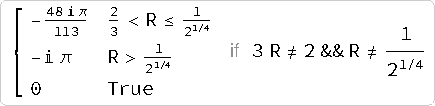
\includegraphics[height=2cm]{img/ContourIntegrate.pdf}
\end{minipage}
\noindent
\mma 按照$R$的不同值给出了不同结果。如果需要提取上面的结果表达式,可以用\verb|InputForm|查看上述内容的具体表达式,再使用\verb|Part|函数提取。再比如,计算一个复平面的上半部分闭合的围道积分,从实轴上半绕过极点 -2,从实轴下半绕过极点 2:

\verb|In[5]:=ContourIntegrate[I E^(-I p)/(p^2 - 4), p | $\in$ \verb| {"UpperSemicircle", 2, -2}]|

\verb|Out[5]=|$-\frac{1}{2} \text{e}^\text{-2 I} \pi$   
\\

\textbf{13.渐进计算}

在版本11.3以及后续版本中,\mma 陆续引入了一系列渐进计算的函数,包括 \verb|Asymptotic|、\verb|AsymptoticIntegrate|、\verb|AsymptoticSum|~等,具体可以参考帮助文档\href{http://reference.wolfram.com/language/guide/Asymptotics.html}{guide/Asymptotics}。例如在无穷远处展开$\Gamma(x)$的首项:

\verb|In[1]:=Asymptotic[Gamma[x], {x, Infinity, 1}]|

\verb|Out[1]=|$\text{e}^{-x}\sqrt{2\pi}x^{-\frac{1}{2}+x}$

在$x=0$处展开$\frac{\sin(x)}{1+x}$到无穷阶:

\verb|In[2]:=Asymptotic[Sin[x]/(1 + x), {x, 0,Infinity}]| 

\noindent
\begin{minipage}[c]{0.1cm}
\verb|    Out[2]=|
\\\\
\end{minipage}
\hfill
\begin{minipage}[b]{14.3cm}\parindent=2\ccwd
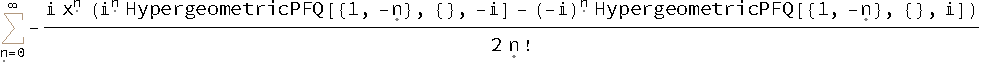
\includegraphics[height=0.94cm]{img/Asymptotic.pdf}
\end{minipage}

计算$x^x$的积分在$x=0$处的渐进展开到2阶:

\verb|In[3]:=AsymptoticIntegrate[x^x, x, {x, 0, 2}]|   

\verb|Out[3]=| $x+\frac{1}{4}x^2(-1+\text{2 Log[}x])$  

计算$\sum_{k=1}^n \frac{1}{k}$ 在 $n=\infty$ 处的展开到2阶:

\verb|In[4]:=AsymptoticSum[1/k, {k, 1, n}, {n, Infinity, 2}]|

\verb|Out[4]=EulerGamma-|$\frac{1}{12n^2}+\frac{1}{2n}+\text{Log[}n]$

更多的使用方法参考具体函数的帮助文档。




\section{Mathematica中的绘图}


这里讲Mathematica中简单的函数可视化。

正如前面所说,Mathematica里面所有对象都是表达式,图形也是。虽然在前端是一个图形,但是内核处理和传递到前端是
都是表达式。Mathematica中图形表达式对结构详见帮助文档
\href{http://reference.wolfram.com/language/tutorial/TheStructureOfGraphicsAndSoundOverview.html}{tutorial/TheStructureOfGraphicsAndSoundOverview}
,至于数据可视化以及使用低级函数~\verb|Graphics|~或~\verb|Graphics3D|画图不在此处讨论范围之列。

应该说,Mathematica中函数可视化是所有数学软件中最简单的,只需要给定要作图的函数以及作图的区域,输入对应的
表达式,剩下的工作Mathematica都会自动完成,比如:

\verb|In[1]:=Plot[Sin[x], {x, 0, 2 Pi}]|

\noindent
\begin{minipage}[b]{0.9cm}%\vskip-8mm
\verb|    Out[1]=|
\\\\\\\\%为了调纵向居中,我才不会告诉你我试了半天最终以四个回车解决了:)
\end{minipage}
\hfill
\begin{minipage}[b]{14.4cm}\parindent=2\ccwd
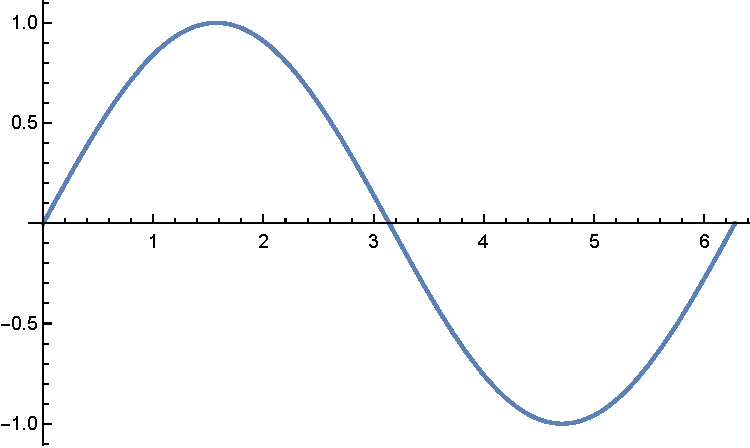
\includegraphics[height=4cm]{img/Sinx.pdf}
\end{minipage}

与函数可视化有关的所有函数在帮助文档
\href{http://reference.wolfram.com/language/guide/FunctionVisualization.html}{guide/FunctionVisualization}
处,以下来做简明介绍。

通常Mathematica用于绘图的函数的选项用于指定绘图的样式,而且一般画同一类型图形的函数选项绝大部分都是一样的,举例时只以一个函数为例。

\subsection{二维绘图}

最基本的画一元函数图形的函数是Plot,具体用法请查询帮助文档,此处仅举几例,如绘制$\Gamma(x)$在\verb|(-5,5)|内的图像:

% \verb|Plot[Gamma[x], {x, -5, 5}]|
\begin{lstlisting}
Plot[Gamma[x], {x, -5, 5}]
\end{lstlisting}

或者是同时绘制几个函数的图像:

% \verb|Plot[{Sin[x], Cos[x], Tan[x]}, {x, -2 Pi, 2 Pi}]|
\begin{lstlisting}
Plot[{Sin[x], Cos[x], Tan[x]}, {x, -2 Pi, 2 Pi}]
\end{lstlisting}

函数Plot的选项是及其多的,共有128个,绝大部分选项看名称就知道作用,比如 ~\verb|AspectRatio|
控制图像的宽高比,~\verb|AxesOrigin|~控制图像坐标轴原点位置,~\verb|PlotRange|~控制绘图范围等。选项
的作用可以参阅~\verb|Plot|~的帮助文档,当然也可以去选项的帮助文档单独查看某个选项的具体使用方法,
如:

% \verb|Plot[Gamma[x], {x, -5, 5}, PlotRange -> {-10, 10}, PlotLabel -> Style[Gamma[x],|\\
% \verb| Black, Bold, 16], AxesStyle -> Directive[Arrowheads[0.03], Italic, Thick], |\\
% \verb|AxesLabel -> (Style[#, Black, Bold, 16] & /@ {x, y}), ColorFunction -> Hue]|

\begin{lstlisting}
Plot[Gamma[x], {x, -5, 5}, PlotRange -> {-10, 10}, 
 PlotLabel -> Style[Gamma[x], Black, Bold, 16], 
 AxesStyle -> Directive[Arrowheads[0.03], Italic, Thick], 
 AxesLabel -> (Style[#, Black, Bold, 16] & /@ {x, y}), 
 ColorFunction -> Hue]
\end{lstlisting}

由于Mathematica的版本变化,以前4.0版本需要加载额外程序包才能进行的绘图,现在也可以直接绘制了,
比如参数函数绘图,是~\verb|ParametricPlot|:

% \verb|ParametricPlot[{Sin[u], Sin[2 u]}, {u, 0, 2 Pi}]|
\begin{lstlisting}
ParametricPlot[{Sin[u], Sin[2 u]}, {u, 0, 2 Pi}]
\end{lstlisting}

极坐标绘图,是~\verb|PolarPlot|:

% \verb|PolarPlot[Sin[3 t], {t, 0, Pi}]|
\begin{lstlisting}
PolarPlot[Sin[3 t], {t, 0, Pi}]
\end{lstlisting}

等高线作图,有~\verb|ContourPlot|:

% \verb|ContourPlot[Cos[x] + Cos[y], {x, 0, 4 Pi}, {y, 0, 4 Pi}]|

% \verb|ContourPlot[Cos[x] + Cos[y] == 1/2, {x, 0, 4 Pi}, {y, 0, 4 Pi}]|
\begin{lstlisting}
ContourPlot[Cos[x] + Cos[y], {x, 0, 4 Pi}, {y, 0, 4 Pi}]
ContourPlot[Cos[x] + Cos[y] == 1/2, {x, 0, 4 Pi}, {y, 0, 4 Pi}]
\end{lstlisting}

密度图,有~\verb|DensityPlot|:

% \verb|DensityPlot[Sin[x] Sin[y], {x, -4, 4}, {y, -3, 3}]|
\begin{lstlisting}
DensityPlot[Sin[x] Sin[y], {x, -4, 4}, {y, -3, 3}]
\end{lstlisting}

至于绘制向量图,有~\verb|StreamPlot|(流线图)、\verb|VectorPlot|(矢量图)、\verb|StreamDensityPlot|
(向量场和标量场函数的叠加图)等,不再细述。

\subsection{三维绘图}

最基本的画二元函数图形的函数是\verb|Plot3D|,比如画$\sin(x y)$的图像:

% \verb|Plot3D[Sin[x y],{x,-Pi,Pi},{y,-Pi,Pi}]|
\begin{lstlisting}
Plot3D[Sin[x y],{x,-Pi,Pi},{y,-Pi,Pi}]
\end{lstlisting}

画三维图的选项和画二维图的选项有点区别,比如控制图形比例的选项从二维图的\verb|AspectRatio|
在三维图里就变成了\verb|BoxRatios|等。\verb|Plot3D|~的选项共有103个,详见参考文档。

对于复变函数的图形,由于我们所在的空间只有三维,所以我们只能够分别画出实部和虚部
(或者模和辐角),比如:

% \verb|pic1=Plot3D[Re[Sin[x + I y]], {x, 0, 5 Pi}, {y, 0, 2}, PlotStyle ->Green]|

% \verb|pic2=Plot3D[Im[Sin[x + I y]], {x, 0, 5 Pi}, {y, 0, 2}, PlotStyle -> Pink]|
\begin{lstlisting}
pic1=Plot3D[Re[Sin[x + I y]], {x, 0, 5 Pi}, {y, 0, 2}, PlotStyle ->Green]
pic2=Plot3D[Im[Sin[x + I y]], {x, 0, 5 Pi}, {y, 0, 2}, PlotStyle -> Pink]
Show[pic1,pic2]
\end{lstlisting}
其中~\verb|PlotStyle|是指定图形的样式,这里是设置了颜色;
~\verb|Show|~是把图形合并到一张图片的函数。
但是~\verb|Show|~只能够合并相同维度的图形,比如合并几张二维图或者几张三维图,但是二维图和三维图就不能够合并
在一起。如果有这样的需求的话,就得使用模式匹配或者使用~\verb|Texture|~来拼装图形,这要求对Mathematica掌握的程度比
较高,此处不再细述。
当然,也可以直接在一张图里面同时画实部和虚部,比如

% \verb|Plot3D[{Re[Sin[x + I y]],Im[Sin[x + I y]]}, {x, 0, 5 Pi}, {y, 0, 2}]|
\begin{lstlisting}
Plot3D[{Re[Sin[x + I y]],Im[Sin[x + I y]]}, {x, 0, 5 Pi}, {y, 0, 2}]
\end{lstlisting}
这时候Mathematica就会自动给不同的图着不同的颜色。
若想以等高线图或者密度图的形式画复变函数的图形,可以考虑前面提到的 \verb|ContourPlot| 和 \verb|DensityPlot| ,
如:

% \verb|ContourPlot[Abs[Sin[x + I y]], {x, 0, 5 Pi}, {y, 0, 2}]|
\begin{lstlisting}
ContourPlot[Abs[Sin[x + I y]], {x, 0, 5 Pi}, {y, 0, 2}]
\end{lstlisting}
\verb|ContourPlot|~和~\verb|DensityPlot|~有时会因为采样的原因导致边缘不光滑,如果出现边缘不平滑的情况,
可以添加选项\verb|PlotPoints|,比如:

% \verb|ContourPlot[Abs[Sin[x + I y]], {x, 0, 5 Pi}, {y, 0, 2}, PlotPoints -> 50]|
\begin{lstlisting}
ContourPlot[Abs[Sin[x + I y]], {x, 0, 5 Pi}, {y, 0, 2}, PlotPoints -> 50]
\end{lstlisting}
当然对所有的绘制函数图像的函数,选项\verb|PlotPoints|都是可用的。
此外,由于选项~\verb|ColorFunction|~的存在,我们可以给一个三维图着色,这意味着我们可以用高度和颜色
分别表示复变函数的实部和虚部(或者模和辐角),如:

% \verb|Plot3D[Abs[Sin[x + I y]], {x, 0, 5 Pi}, {y, 0, 2},|\\
% \verb|     ColorFunction ->  Function[{x, y}, Hue[Arg[Sin[x + I y]]/(2 Pi) + 1/2]],|\\
% \verb|     ColorFunctionScaling -> False]|
\begin{lstlisting}
Plot3D[Abs[Sin[x + I y]], {x, 0, 5 Pi}, {y, 0, 2}, 
 ColorFunction -> 
  Function[{x, y}, Hue[Arg[Sin[x + I y]]/(2 Pi) + 1/2]], 
 ColorFunctionScaling -> False]
\end{lstlisting}
这里就用了高度表示模,颜色表示辐角。选项~\verb|ColorFunction|~给出的必须是一个纯函数,这里就是
\lstinline|Function[{x, y}, Hue[Arg[Sin[x + I y]]/(2 Pi) + 1/2]]|,
其中~\verb|Hue[x]|~是用色相表示的颜色,
x的取值为\verb|0~1|之间,由于\verb|Arg|取值为$(-\pi,\pi]$,所以除以$2\pi$再减去\verb|1/2|保证落在
\verb|0~1|之间。注意当使用~\verb|ColorFunction|~指定颜色函数时,要加上选项 \verb|ColorFunctionScaling -> False|
,否则就会把颜色函数的自变量按尺度按比例缩放到0和1之间,得不到我们想要的结果。

画三维图还有其他诸多函数,比如 \verb|ParametricPlot3D| 绘制三维参数曲线或者曲面, \verb|ContourPlot3D|  绘制三维等值面, \verb|SphericalPlot3D| 绘制三维球面图形,
 \verb|RevolutionPlot3D| 绘制三维旋转图形等,详见帮助文档
 \href{http://reference.wolfram.com/language/guide/FunctionVisualization.html}{guide/FunctionVisualization}
 ,不再细述。

除了\mma 内置的绘图函数外,Wolfram 函数库\footnote{\url{https://resources.wolframcloud.com/FunctionRepository/}}里也有一些独立开发者提供的补充函数,使用这里面的函数需要联网。在本课程里比较有用的一个绘图函数是绘制复变函数的黎曼面,这个函数的名称为\verb|RiemannSurfacePlot3D|,其在线文档在\url{https://resources.wolframcloud.com/FunctionRepository/resources/RiemannSurfacePlot3D/}。比如绘制函数$\sqrt{z}$的黎曼面的代码为

% \verb|ResourceFunction["RiemannSurfacePlot3D"][w== Sqrt[z], Re[w], {z, w}]|   
\begin{lstlisting}
ResourceFunction["RiemannSurfacePlot3D"][w== Sqrt[z], Re[w], {z, w}]
\end{lstlisting}
第一次运行的时候需要下载这个函数的源码,运行速度稍慢,之后运行就会变快。更多的黎曼面绘制例子可以参考该函数的在线文档。



\section{Mathematica中的(偏)微分方程}

Mathematica具有很强大的符号和数值解(偏)微分方程的功能,就在这里做简要介绍。而与此有关的函数,主要是\verb|DSolve|
和\verb|NDSolve|。这两个函数的功能非常强大,可以应用于各种场景,具体内容请参考帮助文档,这里只是举例介绍。

\subsection{符号解(DSolve,DSolveValue)}

\verb|In[1]:=Clear["Global`*"]|

解常微分方程:

\verb|In[2]:=DSolve[y''[x] + 2 y'[x] + y[x] == 0, y[x], x]|

\verb|Out[2]={{y[x] ->|$ \text{e}^\text{-x}$\verb| C[1] + |$\text{e}^\text{-x}$ \verb|x C[2]}}|

\verb|C[1]|和\verb|C[2]|是常数,如果把上面的\verb|y[x]|换成\verb|y|的话,返回的就是一个纯函数:

\verb|In[3]:=DSolve[y''[x] + 2 y'[x] + y[x] == 0, y, x]|

\verb|Out[3]={{y -> Function[{x},| $ \text{e}^\text{-x}$\verb| C[1] + |$\text{e}^\text{-x}$ \verb| x C[2]]}}|

这样的好处是可以调用计算的结果,比如我要计算\verb|y[0]|:

\verb|In[4]:=y[0]/.%[[1,1]]|

\verb|Out[4]=C[1]|

或者求导:

\verb|In[5]:=y'[x]/.%%[[1,1]]|

\verb|Out[5]=-| $ \text{e}^\text{-x}$\verb| C[1] + | $ \text{e}^\text{-x}$\verb| C[2] - | $ \text{e}^\text{-x}$\verb| x C[2]|

% 原理是纯函数\verb|Function[{x},| $ \text{e}^\text{-x}$\verb| C[1] + |$\text{e}^\text{-x}$ \verb| x C[2]]|和Mathematica内置的函数比如
% \verb|Sin|或者\verb|Cos|性质都一样,
\verb|y[0]/.%2[[1,1]]|~这个代码首先把~\verb|y[0]|~中的~\verb|y|~替换了变成
\verb|Function[{x},| $ \text{e}^\text{-x}$\verb| C[1] + |$\text{e}^\text{-x}$ \verb| x C[2]][0]|,
然后计算得结果为\verb|C[1]|。

如果用\verb|DSolveValue|的话,就会直接返回计算的结果而不是一个规则,比如:

\verb|In[6]:=DSolveValue[y''[x] + 2 y'[x] + y[x] == 0, y, x]|

\verb|Out[6]:=Function[{x},| $ \text{e}^\text{-x}$\verb| C[1] + |$\text{e}^\text{-x}$ \verb| x C[2]]|

加上边界条件或者初始条件:

\verb|In[7]:=DSolve[{y''[x] + 2 y'[x] + y[x] == 0, y[1] == 1, y'[1] == 1}, y, x]|

\verb|Out[7]={{y -> Function[{x}, |$\text{e}^\text{1 - x}$\verb| (-1 + 2 x)]}}|

对于绝大部分可以解析解的常微分方程,Mathematica都是可以给出解析解的。

偏微分方程:

\verb|In[8]:=DSolve[c^2 D[u[x, t], x, x] - D[u[x, t], t, t] == 0, u[x, t], {x, t}]|

\verb|Out[8]={{u[x, t] -> C[1][t -|$\frac{\text{x}}{\sqrt{\text{c}^2}}$\verb|] + C[2][t +|$\frac{\text{x}}{\sqrt{\text{c}^2}}$\verb|]}}|

这里显示了Mathematica的一个重要特性,那就是如果你没有指定范围,Mathematica中的符号计算默认所有的符号都是复数,所以上面出现了$\sqrt{\text{c}^2}$,
以至于有时候计算出现了~\verb|ConditionalExpression|~而且计算速度较慢,解决的办法是加上一些假设:

\verb|In[9]:=Assuming[c > 0, DSolve[c^2 D[u[x, t], x, x] - D[u[x, t], t, t] == 0, |\\
\verb|      u[x, t], {x, t}]]|

\verb|Out[9]={{u[x, t] -> C[1][t -|$\frac{\text{x}}{\text{c}}$\verb|] + C[2][t +|$\frac{\text{x}}{\text{c}}$\verb|]}}|

当然,这里的~\verb|C[1]|~和~\verb|C[2]|~是任意形式的函数。

也可以指定边界条件和初始条件解偏微分方程:

\verb|In[10]:=DSolve[{Laplacian[u[x, y], {x, y}] == 0, u[0, y] == y, u[a, y] == 0,|\\
\verb|      u[x, 0] == 0, u[x, b] == 0}, u[x,y], {x, 0, a}, {y, 0, b}]|

\verb|Out[10]={{u[x, y] ->|$\underset{\text{K[1]=1}}{\overset{\infty }{\sum }}\frac{2 (-1)^\text{K[1]+1} \text{b} \text{Csch}[\frac{\pi  \text{ a K[1]}}{\text{b}}] \text{Sin} [\frac{\pi  \text{ y K[1]}}{\text{b}}] \text{Sinh} [\frac{\pi  \text{(a-x) K[1]}}{\text{b}}]}{\pi  \text{K[1]}}$\verb|}}|

\verb|In[11]:=DSolve[{D[u[x, t], t, t] - c^2 D[u[x, t], x, x] == 0,|\\
\verb|       u[x, 0] == x (1 - x), (D[u[x, t], t] /. t -> 0) == 0,|\\
\verb|       u[0, t] == 0,  u[1, t] == 0}, u[x,t], {x, t}]|

\verb|Out[11]={{u[x,t] -> |$\underset{\text{K[1]=1}}{\overset{\infty }{\sum }}-\frac{4 \left(-1+(-1)^{\text{K[1]}}\right)\text{Cos}[\pi  \sqrt{\text{c}^2} \text{ t K[1]}] \text{Sin[} \pi  \text{ x K[1]}] }{\pi ^3 \text{K[1]}^3}$\verb|}}|


我们可以通过把求和上限的无穷大替换成有限的数字实现对于求和的截断,如

% ~\verb|% /. Infinity -> 5 // Activate|,
\begin{lstlisting}
% /. Infinity -> 5 // Activate
\end{lstlisting}
其中函数\verb|Activate|的作用是激活给出的解中未激活求和的\verb|Sum|。
在\mma 版本14中,可以用函数~\verb|TruncateSum|~求截断和,如~\verb|TruncateSum[%%, 5]| 
可以给出上述求和前五项之和的表达式。

不过Mathematica解带有初始条件和边界条件的偏微分方程会有些限制,比如所要解的偏微分方程必须是齐次方程,然后自变量只能有
两个,而且必须是矩形区域。
更多符号求解偏微分方程的内容,可以参考帮助文档~\href{http://reference.wolfram.com/language/tutorial/SymbolicSolutionsOfPDEs.html}{tutorial/SymbolicSolutionsOfPDEs}。

\subsection{级数解}

% 在数学软件Maple中,级数解常微分方程是简单的,\verb|dsolve(ODE, y(x),'series')|就可以给出常微分方程的级数解。但在\mma 中,\verb|DSolve|无法指定方法要求给出级数解,不过
我们可以用已知的函数手动求解常微分方程的级数解,以下以常微分方程$y''(x)-6y(x)^2-x=0$, $y'(0)=0, \quad y(0)=1$为例。

首先定义方程和初始条件以及这个微分方程的算符:

\verb|In[1]:=ode = y''[x] - 6 y[x]^2 - x == 0;| 

\verb|In[2]:=init = {y'[0] == 0, y[0] == 1};|

\verb|In[3]:=op = D[#, {x, 2}] - 6 #^2 - x &;|   

接下来,我们设要求解的级数解的表达式为\verb|ys|,通过\verb|Series|函数可以很快写出\verb|ys|的表达式,这里只展开到5项:

\verb|In[4]:=ys = Series[y[x], {x, 0, 5}]|

\verb|Out[4]=|$\text{y}[0]+ \text{y}'[0]\text{x}+\frac{1}{2}  \text{y}''[0]\text{x}^2+\frac{1}{6}  \text{y}^{(3)}[0]\text{x}^3+\frac{1}{24} 
   \text{y}^{(4)}[0]\text{x}^4+\frac{1}{120}  \text{y}^{(5)}[0]\text{x}^5+\text{O}[\text{x}^6]$

接下来,我们将\verb|ys|的表达式带入方程,再加上初始条件,用函数\verb|SolveAlways|求解,得到

\verb|In[5]:=sol = SolveAlways[Join[{op[ys] == 0}, init], x]|

\verb|Out[5]={{y|$^{(4)}$\verb|[0]->72,y|$^{(5)}$\verb|[0]->12,y|$^{(3)}$\verb|[0]->1,y''[0]->6,y'[0]->0,y[0]->1}}|

将上面的结果带入\verb|ys|的表达式,即可得到方程的级数解

\verb|In[6]:=ys /. sol[[1]]|

\verb|Out[6]=|$1+3 \text{x}^2+\frac{\text{x}^3}{6}+3 \text{x}^4+\frac{\text{x}^5}{10}+\text{O}[\text{x}^6]$

可以将上述求解思路打包成一个函数:
\begin{lstlisting}
ODESeriesSolution[ode_Equal, inits_List, y_, x_, order_ : 5] := 
 Block[{ys, equation, sol},
  ys = Series[y[x], {x, 0, order}];
  equation = ode /. y -> (Evaluate[ys /. x -> #] &);
  sol = SolveAlways[Join[{equation}, inits], x];
  ys /. sol // First
  ]

ODESeriesSolution[y''[x]-6 y[x]^2-x == 0, {y'[0]==0, y[0]==1}, y, x, 20]

ODESeriesSolution[y''[x]-6 y[x]^2-x == 0, {}, y, x, 5]
\end{lstlisting}

在引入了渐进求解的函数之后,级数解微分方程也可以通过\verb|AsymptoticDSolveValue|求解,比如上述方程求解为

\verb|In[7]:=AsymptoticDSolveValue[{ode, init}, y[x], {x, 0, 5}]|

\verb|Out[7]=|$1+3 \text{x}^2+\frac{\text{x}^3}{6}+3 \text{x}^4+\frac{\text{x}^5}{10}$

\subsection{数值解(NDSolve,NDSolveValue)}

\mma 具有强大的数值解微分方程的能力,以下为简要介绍。

% \verb|In[1]:=Clear["Global`*"]|
Mathematica可以求解几乎所有类型的常微分方程组,不过
数值求解微分方程必须要求求解的区域是有限的,而且要求除了自变量外,所有参数都是具体的数,而且必须给定能够唯一确定方程解
的初始条件和边界条件。对于常微分方程的数值解,写法和微分方程基本一样,只是要加上求解区域:

% \verb|In[2]:=sol=NDSolveValue[{y''[x] + 2 y'[x] + y[x] == 0, y[1] == 1,|\\
% \verb|      y'[1] == 1}, y, {x, 1, 10}]|

% \noindent
% \begin{minipage}[b]{1.4cm}%\vskip-8mm
% \verb|    Out[2]=|
% \\
% \end{minipage}
% \hfill
% \begin{minipage}[b]{16.1cm}\parindent=2\ccwd
% 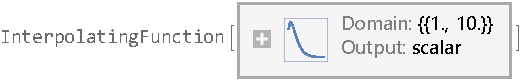
\includegraphics[height=1.1cm]{img/NDSolveValue.pdf}
% \end{minipage}

\begin{lstlisting}
Clear["Global`*"]
sol=NDSolveValue[{y''[x] + 2 y'[x] + y[x] == 0, y[1] == 1,
    y'[1] == 1}, y, {x, 1, 10}]
\end{lstlisting}
所得到的是一个纯函数,如果想要求在某一点的值的话,可以这样:

% \verb|In[3]:=sol[2]|

% \verb|Out[3]=1.10364|
\begin{lstlisting}
sol[2]
(*1.10364*)
\end{lstlisting}
或者绘图:

% \verb|In[4]:=Plot[sol[x], {x, 1, 10}]|
\begin{lstlisting}
Plot[sol[x], {x, 1, 10}]
\end{lstlisting}

然而有时候在数值解常微分方程(组)的时候,可能会因为方程(组)的特性导致求解失败,比如方程(组)是刚性的,或者是求解过程中遇到了
方程的奇点。这时候可以添加选项\verb|Method|来指定针对特定类型的常微分方程(组)的算法,相关内容比较庞大,想深入了解的话需要知道
常微分方程的算法,至于\mma 中对于\verb|NDSolve|的选项说明和一些算法注释可以参考帮助文档
\href{http://reference.wolfram.com/language/tutorial/NDSolveOverview.html}{tutorial/NDSolveOverview}
,不再细述。


如果是数值解偏微分方程的话,情况就有点复杂。目前Mathematica可以解二阶线性偏微分方程组,至于一些非线性的方程有时候会求解失败。
Mathematica版本10.0以后引入了函数狄利克雷条件(\verb|DirichletCondition|)和诺依曼边值(\verb|NeumannValue|),数值解偏微分方程的
边界条件必须由这两个函数指定。而且因为这两个函数的存在,Mathematica中的偏微分方程可以在任意形状区域内数值求解。而且现在Mathematica内置了
有限元程序包,可以使用有限元方法求解偏微分方程,详见帮助文档
\href{http://reference.wolfram.com/language/FEMDocumentation/tutorial/FiniteElementOverview.html}{FEMDocumentation/tutorial/FiniteElementOverview}
,内容过于庞大,不再细述。以下以一个矩形区域的波动方程为例。

一均匀各向同性弹性薄膜,$0\leq x \leq1$,$0\leq y \leq1$,四周夹紧.初始位移为 $xy(1-x)(1-y)$,初始速度为0,波速
为1,求解这个系统。

首先求解这个方程:

% \verb|In[5]:=sol = NDSolveValue[{D[u[t, x, y], t, t] - Laplacian[u[t, x, y], {x, y}] == 0,|\\
% \verb|      u[0, x, y] == x y (1 - x) (1 - y), Derivative[1, 0, 0][u][0, x, y] == 0,|\\
% \verb|      DirichletCondition[u[t, x, y] == 0, True]}, u, {t, 0, 10},  Element[{x, y}, |\\
% \verb|      Rectangle[{0, 0}, {1, 1}]], Method -> {"PDEDiscretization" -> {"MethodOfLines",|\\
% \verb|      "SpatialDiscretization" -> {"FiniteElement"}}}]|
\begin{lstlisting}
sol = NDSolveValue[{D[u[t, x, y], t, t] - Laplacian[u[t, x, y], {x, y}] == 0, u[0, x, y] == x y (1 - x) (1 - y), Derivative[1, 0, 0][u][0, x, y] == 0, DirichletCondition[u[t, x, y] == 0, True]}, u, {t, 0, 10}, Element[{x, y}, Rectangle[{0, 0}, {1, 1}]], Method -> {"PDEDiscretization" -> {"MethodOfLines", "SpatialDiscretization" -> {"FiniteElement"}}}]
\end{lstlisting}
这里就在选项里设定了方法为有限元,计算得到的\verb|sol[t,x,y]|就是方程的解,为了可视化结果,我们可以先画出不同时刻的图像的列表,然后把这个列表中的图片做成动画:

% \verb|In[6]:=list = Table[Plot3D[sol[t, x, y], {x, 0, 1}, {y, 0, 1}, AxesOrigin -> |\\
% \verb|       {0, 0, 0}, Boxed -> False, SphericalRegion -> True,|\\
% \verb|       PlotRange -> {{0, 1}, {0, 1}, {-1/12, 1/12}}], {t, 0, 10, 0.1}];|
\begin{lstlisting}
list = Table[Plot3D[sol[t, x, y], {x, 0, 1}, {y, 0, 1}, AxesOrigin ->{0, 0, 0}, Boxed -> False, SphericalRegion -> True, PlotRange -> {{0, 1}, {0, 1}, {-1/12, 1/12}}], {t, 0, 10, 0.1}];
ListAnimate[list]

\end{lstlisting}


% \verb|In[7]:=ListAnimate[list]|
\noindent
或者导出为gif文件:

% \verb|In[8]:=SetDirectory@NotebookDirectory[];Export["wave.gif", list]|
\begin{lstlisting}
SetDirectory@NotebookDirectory[];
Export["wave.gif", list]
\end{lstlisting}
以上内容涉及Mathematica的许多内容比如列表操作以及文件导入导出等,这里只举了一个例子,有兴趣的同学
可以查询以上代码里面所涉及到的函数。而且Mathematica中求解的区域可以是一些简单规则区域的组合,也可以是随便得到的一个区域,限于篇幅不再细述。

当然Mathematica还有其他的求解(偏)微分方程的函数,比如求解格林函数(\verb|GreenFunction|),求解微分方程的特征函数和特征值
(\verb|DEigensystem|),详见帮助文档,不再细述。




\end{document}